\documentclass[1p]{elsarticle_modified}
%\bibliographystyle{elsarticle-num}

%\usepackage[colorlinks]{hyperref}
%\usepackage{abbrmath_seonhwa} %\Abb, \Ascr, \Acal ,\Abf, \Afrak
\usepackage{amsfonts}
\usepackage{amssymb}
\usepackage{amsmath}
\usepackage{amsthm}
\usepackage{scalefnt}
\usepackage{amsbsy}
\usepackage{kotex}
\usepackage{caption}
\usepackage{subfig}
\usepackage{color}
\usepackage{graphicx}
\usepackage{xcolor} %% white, black, red, green, blue, cyan, magenta, yellow
\usepackage{float}
\usepackage{setspace}
\usepackage{hyperref}

\usepackage{tikz}
\usetikzlibrary{arrows}

\usepackage{multirow}
\usepackage{array} % fixed length table
\usepackage{hhline}

%%%%%%%%%%%%%%%%%%%%%
\makeatletter
\renewcommand*\env@matrix[1][\arraystretch]{%
	\edef\arraystretch{#1}%
	\hskip -\arraycolsep
	\let\@ifnextchar\new@ifnextchar
	\array{*\c@MaxMatrixCols c}}
\makeatother %https://tex.stackexchange.com/questions/14071/how-can-i-increase-the-line-spacing-in-a-matrix
%%%%%%%%%%%%%%%

\usepackage[normalem]{ulem}

\newcommand{\msout}[1]{\ifmmode\text{\sout{\ensuremath{#1}}}\else\sout{#1}\fi}
%SOURCE: \msout is \stkout macro in https://tex.stackexchange.com/questions/20609/strikeout-in-math-mode

\newcommand{\cancel}[1]{
	\ifmmode
	{\color{red}\msout{#1}}
	\else
	{\color{red}\sout{#1}}
	\fi
}

\newcommand{\add}[1]{
	{\color{blue}\uwave{#1}}
}

\newcommand{\replace}[2]{
	\ifmmode
	{\color{red}\msout{#1}}{\color{blue}\uwave{#2}}
	\else
	{\color{red}\sout{#1}}{\color{blue}\uwave{#2}}
	\fi
}

\newcommand{\Sol}{\mathcal{S}} %segment
\newcommand{\D}{D} %diagram
\newcommand{\A}{\mathcal{A}} %arc


%%%%%%%%%%%%%%%%%%%%%%%%%%%%%5 test

\def\sl{\operatorname{\textup{SL}}(2,\Cbb)}
\def\psl{\operatorname{\textup{PSL}}(2,\Cbb)}
\def\quan{\mkern 1mu \triangleright \mkern 1mu}

\theoremstyle{definition}
\newtheorem{thm}{Theorem}[section]
\newtheorem{prop}[thm]{Proposition}
\newtheorem{lem}[thm]{Lemma}
\newtheorem{ques}[thm]{Question}
\newtheorem{cor}[thm]{Corollary}
\newtheorem{defn}[thm]{Definition}
\newtheorem{exam}[thm]{Example}
\newtheorem{rmk}[thm]{Remark}
\newtheorem{alg}[thm]{Algorithm}

\newcommand{\I}{\sqrt{-1}}
\begin{document}

%\begin{frontmatter}
%
%\title{Boundary parabolic representations of knots up to 8 crossings}
%
%%% Group authors per affiliation:
%\author{Yunhi Cho} 
%\address{Department of Mathematics, University of Seoul, Seoul, Korea}
%\ead{yhcho@uos.ac.kr}
%
%
%\author{Seonhwa Kim} %\fnref{s_kim}}
%\address{Center for Geometry and Physics, Institute for Basic Science, Pohang, 37673, Korea}
%\ead{ryeona17@ibs.re.kr}
%
%\author{Hyuk Kim}
%\address{Department of Mathematical Sciences, Seoul National University, Seoul 08826, Korea}
%\ead{hyukkim@snu.ac.kr}
%
%\author{Seokbeom Yoon}
%\address{Department of Mathematical Sciences, Seoul National University, Seoul, 08826,  Korea}
%\ead{sbyoon15@snu.ac.kr}
%
%\begin{abstract}
%We find all boundary parabolic representation of knots up to 8 crossings.
%
%\end{abstract}
%\begin{keyword}
%    \MSC[2010] 57M25 
%\end{keyword}
%
%\end{frontmatter}

%\linenumbers
%\tableofcontents
%
\newcommand\colored[1]{\textcolor{white}{\rule[-0.35ex]{0.8em}{1.4ex}}\kern-0.8em\color{red} #1}%
%\newcommand\colored[1]{\textcolor{white}{ #1}\kern-2.17ex	\textcolor{white}{ #1}\kern-1.81ex	\textcolor{white}{ #1}\kern-2.15ex\color{red}#1	}

{\Large $\underline{12a_{0479}~(K12a_{0479})}$}

\setlength{\tabcolsep}{10pt}
\renewcommand{\arraystretch}{1.6}
\vspace{1cm}\begin{tabular}{m{100pt}>{\centering\arraybackslash}m{274pt}}
\multirow{5}{120pt}{
	\centering
	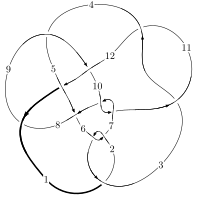
\includegraphics[width=112pt]{../../../GIT/diagram.site/Diagrams/png/1280_12a_0479.png}\\
\ \ \ A knot diagram\footnotemark}&
\allowdisplaybreaks
\textbf{Linearized knot diagam} \\
\cline{2-2}
 &
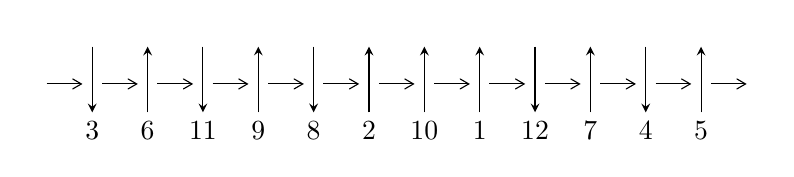
\begin{tikzpicture}[x=20pt, y=17pt]
	% nodes
	\node (C0) at (0, 0) {};
	\node (C1) at (1, 0) {};
	\node (C1U) at (1, +1) {};
	\node (C1D) at (1, -1) {3};

	\node (C2) at (2, 0) {};
	\node (C2U) at (2, +1) {};
	\node (C2D) at (2, -1) {6};

	\node (C3) at (3, 0) {};
	\node (C3U) at (3, +1) {};
	\node (C3D) at (3, -1) {11};

	\node (C4) at (4, 0) {};
	\node (C4U) at (4, +1) {};
	\node (C4D) at (4, -1) {9};

	\node (C5) at (5, 0) {};
	\node (C5U) at (5, +1) {};
	\node (C5D) at (5, -1) {8};

	\node (C6) at (6, 0) {};
	\node (C6U) at (6, +1) {};
	\node (C6D) at (6, -1) {2};

	\node (C7) at (7, 0) {};
	\node (C7U) at (7, +1) {};
	\node (C7D) at (7, -1) {10};

	\node (C8) at (8, 0) {};
	\node (C8U) at (8, +1) {};
	\node (C8D) at (8, -1) {1};

	\node (C9) at (9, 0) {};
	\node (C9U) at (9, +1) {};
	\node (C9D) at (9, -1) {12};

	\node (C10) at (10, 0) {};
	\node (C10U) at (10, +1) {};
	\node (C10D) at (10, -1) {7};

	\node (C11) at (11, 0) {};
	\node (C11U) at (11, +1) {};
	\node (C11D) at (11, -1) {4};

	\node (C12) at (12, 0) {};
	\node (C12U) at (12, +1) {};
	\node (C12D) at (12, -1) {5};
	\node (C13) at (13, 0) {};

	% arrows
	\draw[->,>={angle 60}]
	(C0) edge (C1) (C1) edge (C2) (C2) edge (C3) (C3) edge (C4) (C4) edge (C5) (C5) edge (C6) (C6) edge (C7) (C7) edge (C8) (C8) edge (C9) (C9) edge (C10) (C10) edge (C11) (C11) edge (C12) (C12) edge (C13) ;	\draw[->,>=stealth]
	(C1U) edge (C1D) (C2D) edge (C2U) (C3U) edge (C3D) (C4D) edge (C4U) (C5U) edge (C5D) (C6D) edge (C6U) (C7D) edge (C7U) (C8D) edge (C8U) (C9U) edge (C9D) (C10D) edge (C10U) (C11U) edge (C11D) (C12D) edge (C12U) ;
	\end{tikzpicture} \\
\hhline{~~} \\& 
\textbf{Solving Sequence} \\ \cline{2-2} 
 &
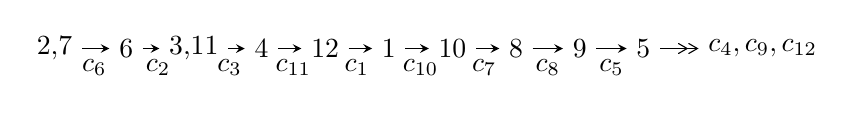
\begin{tikzpicture}[x=23pt, y=7pt]
	% node
	\node (A0) at (-1/8, 0) {2,7};
	\node (A1) at (1, 0) {6};
	\node (A2) at (33/16, 0) {3,11};
	\node (A3) at (25/8, 0) {4};
	\node (A4) at (33/8, 0) {12};
	\node (A5) at (41/8, 0) {1};
	\node (A6) at (49/8, 0) {10};
	\node (A7) at (57/8, 0) {8};
	\node (A8) at (65/8, 0) {9};
	\node (A9) at (73/8, 0) {5};
	\node (C1) at (1/2, -1) {$c_{6}$};
	\node (C2) at (3/2, -1) {$c_{2}$};
	\node (C3) at (21/8, -1) {$c_{3}$};
	\node (C4) at (29/8, -1) {$c_{11}$};
	\node (C5) at (37/8, -1) {$c_{1}$};
	\node (C6) at (45/8, -1) {$c_{10}$};
	\node (C7) at (53/8, -1) {$c_{7}$};
	\node (C8) at (61/8, -1) {$c_{8}$};
	\node (C9) at (69/8, -1) {$c_{5}$};
	\node (A10) at (11, 0) {$c_{4},c_{9},c_{12}$};

	% edge
	\draw[->,>=stealth]	
	(A0) edge (A1) (A1) edge (A2) (A2) edge (A3) (A3) edge (A4) (A4) edge (A5) (A5) edge (A6) (A6) edge (A7) (A7) edge (A8) (A8) edge (A9) ;
	\draw[->>,>={angle 60}]	
	(A9) edge (A10);
\end{tikzpicture} \\ 

\end{tabular} \\

\footnotetext{
The image of knot diagram is generated by the software ``\textbf{Draw programme}" developed by Andrew Bartholomew(\url{http://www.layer8.co.uk/maths/draw/index.htm\#Running-draw}), where we modified some parts for our purpose(\url{https://github.com/CATsTAILs/LinksPainter}).
}\phantom \\ \newline 
\centering \textbf{Ideals for irreducible components\footnotemark of $X_{\text{par}}$} 
 
\begin{align*}
I^u_{1}&=\langle 
2.96804\times10^{545} u^{169}+2.05449\times10^{545} u^{168}+\cdots+3.04382\times10^{547} b-9.96636\times10^{547},\\
\phantom{I^u_{1}}&\phantom{= \langle  }7.76117\times10^{548} u^{169}+3.65178\times10^{548} u^{168}+\cdots+1.18100\times10^{550} a-1.73137\times10^{551},\\
\phantom{I^u_{1}}&\phantom{= \langle  }u^{170}+u^{169}+\cdots-161 u+97\rangle \\
I^u_{2}&=\langle 
188679637611 u^{37}+583203930928 u^{36}+\cdots+19303084121 b-114942573145,\\
\phantom{I^u_{2}}&\phantom{= \langle  }-162853256113 u^{37}-474271015058 u^{36}+\cdots+19303084121 a+168572690127,\\
\phantom{I^u_{2}}&\phantom{= \langle  }u^{38}+4 u^{37}+\cdots- u+1\rangle \\
I^u_{3}&=\langle 
b+1,\;2 a^2-4 a u+5 a-4 u+2,\;u^2- u+1\rangle \\
\\
\end{align*}
\raggedright * 3 irreducible components of $\dim_{\mathbb{C}}=0$, with total 212 representations.\\
\footnotetext{All coefficients of polynomials are rational numbers. But the coefficients are sometimes approximated in decimal forms when there is not enough margin.}
\newpage
\renewcommand{\arraystretch}{1}
\centering \section*{I. $I^u_{1}= \langle 2.97\times10^{545} u^{169}+2.05\times10^{545} u^{168}+\cdots+3.04\times10^{547} b-9.97\times10^{547},\;7.76\times10^{548} u^{169}+3.65\times10^{548} u^{168}+\cdots+1.18\times10^{550} a-1.73\times10^{551},\;u^{170}+u^{169}+\cdots-161 u+97 \rangle$}
\flushleft \textbf{(i) Arc colorings}\\
\begin{tabular}{m{7pt} m{180pt} m{7pt} m{180pt} }
\flushright $a_{2}=$&$\begin{pmatrix}0\\u\end{pmatrix}$ \\
\flushright $a_{7}=$&$\begin{pmatrix}1\\0\end{pmatrix}$ \\
\flushright $a_{6}=$&$\begin{pmatrix}1\\u^2\end{pmatrix}$ \\
\flushright $a_{3}=$&$\begin{pmatrix}u\\u^3+u\end{pmatrix}$ \\
\flushright $a_{11}=$&$\begin{pmatrix}-0.0657169 u^{169}-0.0309210 u^{168}+\cdots-14.6441 u+14.6602\\-0.00975105 u^{169}-0.00674973 u^{168}+\cdots-10.8483 u+3.27430\end{pmatrix}$ \\
\flushright $a_{4}=$&$\begin{pmatrix}0.130093 u^{169}-0.0228900 u^{168}+\cdots+38.5644 u-25.8712\\-0.0700178 u^{169}-0.0639308 u^{168}+\cdots-16.7075 u+4.79517\end{pmatrix}$ \\
\flushright $a_{12}=$&$\begin{pmatrix}-0.0983533 u^{169}-0.457517 u^{168}+\cdots+16.4302 u-26.7107\\-0.0737470 u^{169}-0.0592229 u^{168}+\cdots-23.1395 u+9.10530\end{pmatrix}$ \\
\flushright $a_{1}=$&$\begin{pmatrix}u^3\\u^5+u^3+u\end{pmatrix}$ \\
\flushright $a_{10}=$&$\begin{pmatrix}-0.0559659 u^{169}-0.0241713 u^{168}+\cdots-3.79580 u+11.3859\\-0.00975105 u^{169}-0.00674973 u^{168}+\cdots-10.8483 u+3.27430\end{pmatrix}$ \\
\flushright $a_{8}=$&$\begin{pmatrix}-0.0613740 u^{169}-0.198434 u^{168}+\cdots+7.60465 u-16.2775\\0.0182553 u^{169}+0.0776958 u^{168}+\cdots+5.25855 u+5.73569\end{pmatrix}$ \\
\flushright $a_{9}=$&$\begin{pmatrix}-0.0756754 u^{169}-0.177887 u^{168}+\cdots+1.02654 u-11.6728\\0.0239517 u^{169}+0.0570506 u^{168}+\cdots+10.1931 u+1.76379\end{pmatrix}$ \\
\flushright $a_{5}=$&$\begin{pmatrix}0.119936 u^{169}+0.0216596 u^{168}+\cdots+43.5327 u-20.6550\\-0.0368181 u^{169}-0.0402453 u^{168}+\cdots-15.5079 u+7.91941\end{pmatrix}$\\&\end{tabular}
\flushleft \textbf{(ii) Obstruction class $= -1$}\\~\\
\flushleft \textbf{(iii) Cusp Shapes $= 0.238835 u^{169}+0.220894 u^{168}+\cdots+102.782 u-13.6065$}\\~\\
\newpage\renewcommand{\arraystretch}{1}
\flushleft \textbf{(iv) u-Polynomials at the component}\newline \\
\begin{tabular}{m{50pt}|m{274pt}}
Crossings & \hspace{64pt}u-Polynomials at each crossing \\
\hline $$\begin{aligned}c_{1}\end{aligned}$$&$\begin{aligned}
&u^{170}+87 u^{169}+\cdots+301939 u+9409
\end{aligned}$\\
\hline $$\begin{aligned}c_{2},c_{6}\end{aligned}$$&$\begin{aligned}
&u^{170}+u^{169}+\cdots-161 u+97
\end{aligned}$\\
\hline $$\begin{aligned}c_{3},c_{11}\end{aligned}$$&$\begin{aligned}
&4(4 u^{170}+14 u^{169}+\cdots+1.07793\times10^{8} u+1.77021\times10^{7})
\end{aligned}$\\
\hline $$\begin{aligned}c_{4}\end{aligned}$$&$\begin{aligned}
&u^{170}-2 u^{169}+\cdots+117766 u+85948
\end{aligned}$\\
\hline $$\begin{aligned}c_{5}\end{aligned}$$&$\begin{aligned}
&4(4 u^{170}-38 u^{169}+\cdots-373833 u+44333)
\end{aligned}$\\
\hline $$\begin{aligned}c_{7},c_{10}\end{aligned}$$&$\begin{aligned}
&u^{170}-10 u^{169}+\cdots+214205 u+28225
\end{aligned}$\\
\hline $$\begin{aligned}c_{8}\end{aligned}$$&$\begin{aligned}
&u^{170}-4 u^{169}+\cdots+550206 u+30733
\end{aligned}$\\
\hline $$\begin{aligned}c_{9}\end{aligned}$$&$\begin{aligned}
&u^{170}-10 u^{169}+\cdots-1952 u+256
\end{aligned}$\\
\hline $$\begin{aligned}c_{12}\end{aligned}$$&$\begin{aligned}
&4(4 u^{170}-2 u^{169}+\cdots-30 u+25)
\end{aligned}$\\
\hline
\end{tabular}\\~\\
\newpage\renewcommand{\arraystretch}{1}
\flushleft \textbf{(v) Riley Polynomials at the component}\newline \\
\begin{tabular}{m{50pt}|m{274pt}}
Crossings & \hspace{64pt}Riley Polynomials at each crossing \\
\hline $$\begin{aligned}c_{1}\end{aligned}$$&$\begin{aligned}
&y^{170}+7 y^{169}+\cdots-8189301629 y+88529281
\end{aligned}$\\
\hline $$\begin{aligned}c_{2},c_{6}\end{aligned}$$&$\begin{aligned}
&y^{170}+87 y^{169}+\cdots+301939 y+9409
\end{aligned}$\\
\hline $$\begin{aligned}c_{3},c_{11}\end{aligned}$$&$\begin{aligned}
&16\\
&\cdot(16 y^{170}-1900 y^{169}+\cdots-9315973042219045 y+313365654366769)
\end{aligned}$\\
\hline $$\begin{aligned}c_{4}\end{aligned}$$&$\begin{aligned}
&y^{170}+30 y^{169}+\cdots+522801654484 y+7387058704
\end{aligned}$\\
\hline $$\begin{aligned}c_{5}\end{aligned}$$&$\begin{aligned}
&16(16 y^{170}-188 y^{169}+\cdots+1.20542\times10^{11} y+1.96541\times10^{9})
\end{aligned}$\\
\hline $$\begin{aligned}c_{7},c_{10}\end{aligned}$$&$\begin{aligned}
&y^{170}+100 y^{169}+\cdots-20975614675 y+796650625
\end{aligned}$\\
\hline $$\begin{aligned}c_{8}\end{aligned}$$&$\begin{aligned}
&y^{170}+58 y^{168}+\cdots+46008453280 y+944517289
\end{aligned}$\\
\hline $$\begin{aligned}c_{9}\end{aligned}$$&$\begin{aligned}
&y^{170}-44 y^{169}+\cdots-1694720 y+65536
\end{aligned}$\\
\hline $$\begin{aligned}c_{12}\end{aligned}$$&$\begin{aligned}
&16(16 y^{170}+116 y^{169}+\cdots-32800 y+625)
\end{aligned}$\\
\hline
\end{tabular}\\~\\
\newpage\flushleft \textbf{(vi) Complex Volumes and Cusp Shapes}
$$\begin{array}{c|c|c}  
\text{Solutions to }I^u_{1}& \I (\text{vol} + \sqrt{-1}CS) & \text{Cusp shape}\\
 \hline 
\begin{aligned}
u &= \phantom{-}0.797900 + 0.612016 I \\
a &= -1.205320 - 0.076243 I \\
b &= -0.594567 - 0.841349 I\end{aligned}
 & \phantom{-}1.98698 + 5.39543 I & \phantom{-0.000000 } 0 \\ \hline\begin{aligned}
u &= \phantom{-}0.797900 - 0.612016 I \\
a &= -1.205320 + 0.076243 I \\
b &= -0.594567 + 0.841349 I\end{aligned}
 & \phantom{-}1.98698 - 5.39543 I & \phantom{-0.000000 } 0 \\ \hline\begin{aligned}
u &= -0.581441 + 0.789817 I \\
a &= \phantom{-}0.740097 + 0.999529 I \\
b &= \phantom{-}1.026310 + 0.233750 I\end{aligned}
 & \phantom{-}3.21054 - 0.83988 I & \phantom{-0.000000 } 0 \\ \hline\begin{aligned}
u &= -0.581441 - 0.789817 I \\
a &= \phantom{-}0.740097 - 0.999529 I \\
b &= \phantom{-}1.026310 - 0.233750 I\end{aligned}
 & \phantom{-}3.21054 + 0.83988 I & \phantom{-0.000000 } 0 \\ \hline\begin{aligned}
u &= \phantom{-}0.324167 + 0.967193 I \\
a &= \phantom{-}1.287070 - 0.516048 I \\
b &= \phantom{-}0.539961 - 0.833775 I\end{aligned}
 & -4.57220 + 0.78663 I & \phantom{-0.000000 } 0 \\ \hline\begin{aligned}
u &= \phantom{-}0.324167 - 0.967193 I \\
a &= \phantom{-}1.287070 + 0.516048 I \\
b &= \phantom{-}0.539961 + 0.833775 I\end{aligned}
 & -4.57220 - 0.78663 I & \phantom{-0.000000 } 0 \\ \hline\begin{aligned}
u &= -0.578263 + 0.842304 I \\
a &= \phantom{-}1.33417 + 0.49401 I \\
b &= \phantom{-}1.033130 - 0.495421 I\end{aligned}
 & \phantom{-}3.04326 - 3.77390 I & \phantom{-0.000000 } 0 \\ \hline\begin{aligned}
u &= -0.578263 - 0.842304 I \\
a &= \phantom{-}1.33417 - 0.49401 I \\
b &= \phantom{-}1.033130 + 0.495421 I\end{aligned}
 & \phantom{-}3.04326 + 3.77390 I & \phantom{-0.000000 } 0 \\ \hline\begin{aligned}
u &= -0.938898 + 0.270582 I \\
a &= -0.478572 - 0.776400 I \\
b &= \phantom{-}0.057674 - 0.971978 I\end{aligned}
 & -3.95788 - 0.27759 I & \phantom{-0.000000 } 0 \\ \hline\begin{aligned}
u &= -0.938898 - 0.270582 I \\
a &= -0.478572 + 0.776400 I \\
b &= \phantom{-}0.057674 + 0.971978 I\end{aligned}
 & -3.95788 + 0.27759 I & \phantom{-0.000000 } 0\\
 \hline 
 \end{array}$$\newpage$$\begin{array}{c|c|c}  
\text{Solutions to }I^u_{1}& \I (\text{vol} + \sqrt{-1}CS) & \text{Cusp shape}\\
 \hline 
\begin{aligned}
u &= \phantom{-}0.904837 + 0.493495 I \\
a &= \phantom{-}0.396656 - 1.299930 I \\
b &= \phantom{-}0.570927 - 1.291670 I\end{aligned}
 & -2.59121 - 5.15101 I & \phantom{-0.000000 } 0 \\ \hline\begin{aligned}
u &= \phantom{-}0.904837 - 0.493495 I \\
a &= \phantom{-}0.396656 + 1.299930 I \\
b &= \phantom{-}0.570927 + 1.291670 I\end{aligned}
 & -2.59121 + 5.15101 I & \phantom{-0.000000 } 0 \\ \hline\begin{aligned}
u &= \phantom{-}0.984340 + 0.309300 I \\
a &= -0.830632 + 0.932118 I \\
b &= -0.61999 + 1.30754 I\end{aligned}
 & -4.1593 - 14.7457 I & \phantom{-0.000000 } 0 \\ \hline\begin{aligned}
u &= \phantom{-}0.984340 - 0.309300 I \\
a &= -0.830632 - 0.932118 I \\
b &= -0.61999 - 1.30754 I\end{aligned}
 & -4.1593 + 14.7457 I & \phantom{-0.000000 } 0 \\ \hline\begin{aligned}
u &= -0.993607 + 0.292160 I \\
a &= -0.806373 - 0.762874 I \\
b &= -0.479331 - 1.176830 I\end{aligned}
 & -5.10233 + 6.25376 I & \phantom{-0.000000 } 0 \\ \hline\begin{aligned}
u &= -0.993607 - 0.292160 I \\
a &= -0.806373 + 0.762874 I \\
b &= -0.479331 + 1.176830 I\end{aligned}
 & -5.10233 - 6.25376 I & \phantom{-0.000000 } 0 \\ \hline\begin{aligned}
u &= -0.753025 + 0.590818 I \\
a &= -1.153680 + 0.005001 I \\
b &= -0.783785 + 0.318003 I\end{aligned}
 & \phantom{-}3.50957 + 3.67877 I & \phantom{-0.000000 } 0 \\ \hline\begin{aligned}
u &= -0.753025 - 0.590818 I \\
a &= -1.153680 - 0.005001 I \\
b &= -0.783785 - 0.318003 I\end{aligned}
 & \phantom{-}3.50957 - 3.67877 I & \phantom{-0.000000 } 0 \\ \hline\begin{aligned}
u &= -0.189212 + 1.033370 I \\
a &= \phantom{-}0.86744 + 2.00621 I \\
b &= -0.214291 - 0.906920 I\end{aligned}
 & -3.87988 + 6.39379 I & \phantom{-0.000000 } 0 \\ \hline\begin{aligned}
u &= -0.189212 - 1.033370 I \\
a &= \phantom{-}0.86744 - 2.00621 I \\
b &= -0.214291 + 0.906920 I\end{aligned}
 & -3.87988 - 6.39379 I & \phantom{-0.000000 } 0\\
 \hline 
 \end{array}$$\newpage$$\begin{array}{c|c|c}  
\text{Solutions to }I^u_{1}& \I (\text{vol} + \sqrt{-1}CS) & \text{Cusp shape}\\
 \hline 
\begin{aligned}
u &= \phantom{-}0.764709 + 0.724926 I \\
a &= \phantom{-}0.516850 + 0.808220 I \\
b &= \phantom{-}0.312404 + 0.909118 I\end{aligned}
 & \phantom{-}0.18493 + 3.40108 I & \phantom{-0.000000 } 0 \\ \hline\begin{aligned}
u &= \phantom{-}0.764709 - 0.724926 I \\
a &= \phantom{-}0.516850 - 0.808220 I \\
b &= \phantom{-}0.312404 - 0.909118 I\end{aligned}
 & \phantom{-}0.18493 - 3.40108 I & \phantom{-0.000000 } 0 \\ \hline\begin{aligned}
u &= \phantom{-}0.071613 + 1.051820 I \\
a &= -0.065299 - 0.411624 I \\
b &= -0.504294 + 0.182751 I\end{aligned}
 & -2.26689 + 3.03836 I & \phantom{-0.000000 } 0 \\ \hline\begin{aligned}
u &= \phantom{-}0.071613 - 1.051820 I \\
a &= -0.065299 + 0.411624 I \\
b &= -0.504294 - 0.182751 I\end{aligned}
 & -2.26689 - 3.03836 I & \phantom{-0.000000 } 0 \\ \hline\begin{aligned}
u &= \phantom{-}0.298186 + 0.890547 I \\
a &= \phantom{-}1.11379 - 2.41741 I \\
b &= \phantom{-}0.184850 + 1.131910 I\end{aligned}
 & -4.27666 + 1.72259 I & \phantom{-0.000000 } 0 \\ \hline\begin{aligned}
u &= \phantom{-}0.298186 - 0.890547 I \\
a &= \phantom{-}1.11379 + 2.41741 I \\
b &= \phantom{-}0.184850 - 1.131910 I\end{aligned}
 & -4.27666 - 1.72259 I & \phantom{-0.000000 } 0 \\ \hline\begin{aligned}
u &= \phantom{-}0.589456 + 0.885556 I \\
a &= -0.566367 + 0.185220 I \\
b &= -0.0880594 - 0.0569484 I\end{aligned}
 & \phantom{-}0.18288 + 2.30892 I & \phantom{-0.000000 } 0 \\ \hline\begin{aligned}
u &= \phantom{-}0.589456 - 0.885556 I \\
a &= -0.566367 - 0.185220 I \\
b &= -0.0880594 + 0.0569484 I\end{aligned}
 & \phantom{-}0.18288 - 2.30892 I & \phantom{-0.000000 } 0 \\ \hline\begin{aligned}
u &= \phantom{-}0.443066 + 0.970162 I \\
a &= \phantom{-}3.32701 - 1.34685 I \\
b &= \phantom{-}0.133369 + 1.031810 I\end{aligned}
 & -3.88542 + 2.24997 I & \phantom{-0.000000 } 0 \\ \hline\begin{aligned}
u &= \phantom{-}0.443066 - 0.970162 I \\
a &= \phantom{-}3.32701 + 1.34685 I \\
b &= \phantom{-}0.133369 - 1.031810 I\end{aligned}
 & -3.88542 - 2.24997 I & \phantom{-0.000000 } 0\\
 \hline 
 \end{array}$$\newpage$$\begin{array}{c|c|c}  
\text{Solutions to }I^u_{1}& \I (\text{vol} + \sqrt{-1}CS) & \text{Cusp shape}\\
 \hline 
\begin{aligned}
u &= \phantom{-}0.558615 + 0.911835 I \\
a &= \phantom{-}0.110603 - 1.344980 I \\
b &= \phantom{-}0.903116 - 0.240646 I\end{aligned}
 & \phantom{-}1.69401 + 1.61828 I & \phantom{-0.000000 } 0 \\ \hline\begin{aligned}
u &= \phantom{-}0.558615 - 0.911835 I \\
a &= \phantom{-}0.110603 + 1.344980 I \\
b &= \phantom{-}0.903116 + 0.240646 I\end{aligned}
 & \phantom{-}1.69401 - 1.61828 I & \phantom{-0.000000 } 0 \\ \hline\begin{aligned}
u &= \phantom{-}0.108200 + 1.073210 I \\
a &= -0.99497 + 1.66194 I \\
b &= -0.537616 - 0.876960 I\end{aligned}
 & -3.95331 + 6.69101 I & \phantom{-0.000000 } 0 \\ \hline\begin{aligned}
u &= \phantom{-}0.108200 - 1.073210 I \\
a &= -0.99497 - 1.66194 I \\
b &= -0.537616 + 0.876960 I\end{aligned}
 & -3.95331 - 6.69101 I & \phantom{-0.000000 } 0 \\ \hline\begin{aligned}
u &= -0.563078 + 0.924351 I \\
a &= -0.933560 - 0.706105 I \\
b &= -0.186770 + 0.972896 I\end{aligned}
 & -0.73731 + 1.67258 I & \phantom{-0.000000 } 0 \\ \hline\begin{aligned}
u &= -0.563078 - 0.924351 I \\
a &= -0.933560 + 0.706105 I \\
b &= -0.186770 - 0.972896 I\end{aligned}
 & -0.73731 - 1.67258 I & \phantom{-0.000000 } 0 \\ \hline\begin{aligned}
u &= -0.245185 + 1.055610 I \\
a &= \phantom{-}1.85232 + 1.00050 I \\
b &= \phantom{-}0.137125 + 0.134857 I\end{aligned}
 & -4.32005 - 7.61029 I & \phantom{-0.000000 } 0 \\ \hline\begin{aligned}
u &= -0.245185 - 1.055610 I \\
a &= \phantom{-}1.85232 - 1.00050 I \\
b &= \phantom{-}0.137125 - 0.134857 I\end{aligned}
 & -4.32005 + 7.61029 I & \phantom{-0.000000 } 0 \\ \hline\begin{aligned}
u &= \phantom{-}0.744599 + 0.500802 I \\
a &= \phantom{-}0.727076 - 0.905652 I \\
b &= \phantom{-}0.582794 + 0.114236 I\end{aligned}
 & -0.743385 - 0.403774 I & \phantom{-0.000000 } 0 \\ \hline\begin{aligned}
u &= \phantom{-}0.744599 - 0.500802 I \\
a &= \phantom{-}0.727076 + 0.905652 I \\
b &= \phantom{-}0.582794 - 0.114236 I\end{aligned}
 & -0.743385 + 0.403774 I & \phantom{-0.000000 } 0\\
 \hline 
 \end{array}$$\newpage$$\begin{array}{c|c|c}  
\text{Solutions to }I^u_{1}& \I (\text{vol} + \sqrt{-1}CS) & \text{Cusp shape}\\
 \hline 
\begin{aligned}
u &= \phantom{-}0.355278 + 1.045980 I \\
a &= \phantom{-}0.748821 - 0.183089 I \\
b &= -0.29888 + 1.82417 I\end{aligned}
 & -9.94153 + 6.24861 I & \phantom{-0.000000 } 0 \\ \hline\begin{aligned}
u &= \phantom{-}0.355278 - 1.045980 I \\
a &= \phantom{-}0.748821 + 0.183089 I \\
b &= -0.29888 - 1.82417 I\end{aligned}
 & -9.94153 - 6.24861 I & \phantom{-0.000000 } 0 \\ \hline\begin{aligned}
u &= -0.837717 + 0.310157 I \\
a &= \phantom{-}0.84255 + 1.18542 I \\
b &= \phantom{-}0.62352 + 1.38908 I\end{aligned}
 & -2.14879 + 6.34317 I & \phantom{-0.000000 } 0 \\ \hline\begin{aligned}
u &= -0.837717 - 0.310157 I \\
a &= \phantom{-}0.84255 - 1.18542 I \\
b &= \phantom{-}0.62352 - 1.38908 I\end{aligned}
 & -2.14879 - 6.34317 I & \phantom{-0.000000 } 0 \\ \hline\begin{aligned}
u &= -0.256258 + 1.080230 I \\
a &= -1.39431 - 1.00857 I \\
b &= -0.244455 + 1.151430 I\end{aligned}
 & -5.99643 + 0.32024 I & \phantom{-0.000000 } 0 \\ \hline\begin{aligned}
u &= -0.256258 - 1.080230 I \\
a &= -1.39431 + 1.00857 I \\
b &= -0.244455 - 1.151430 I\end{aligned}
 & -5.99643 - 0.32024 I & \phantom{-0.000000 } 0 \\ \hline\begin{aligned}
u &= -0.664018 + 0.588943 I \\
a &= -0.340450 + 0.366155 I \\
b &= -0.527929 - 0.695118 I\end{aligned}
 & \phantom{-}0.24571 - 6.49472 I & \phantom{-0.000000 } 0 \\ \hline\begin{aligned}
u &= -0.664018 - 0.588943 I \\
a &= -0.340450 - 0.366155 I \\
b &= -0.527929 + 0.695118 I\end{aligned}
 & \phantom{-}0.24571 + 6.49472 I & \phantom{-0.000000 } 0 \\ \hline\begin{aligned}
u &= \phantom{-}0.143835 + 0.875414 I \\
a &= -0.748366 + 0.585575 I \\
b &= \phantom{-}0.11127 - 1.76500 I\end{aligned}
 & -8.70323 - 4.14735 I & \phantom{-0.000000 } 0 \\ \hline\begin{aligned}
u &= \phantom{-}0.143835 - 0.875414 I \\
a &= -0.748366 - 0.585575 I \\
b &= \phantom{-}0.11127 + 1.76500 I\end{aligned}
 & -8.70323 + 4.14735 I & \phantom{-0.000000 } 0\\
 \hline 
 \end{array}$$\newpage$$\begin{array}{c|c|c}  
\text{Solutions to }I^u_{1}& \I (\text{vol} + \sqrt{-1}CS) & \text{Cusp shape}\\
 \hline 
\begin{aligned}
u &= \phantom{-}0.479555 + 1.005950 I \\
a &= \phantom{-}1.07109 - 1.05115 I \\
b &= \phantom{-}1.62018 - 0.29861 I\end{aligned}
 & -0.51289 + 2.95844 I & \phantom{-0.000000 } 0 \\ \hline\begin{aligned}
u &= \phantom{-}0.479555 - 1.005950 I \\
a &= \phantom{-}1.07109 + 1.05115 I \\
b &= \phantom{-}1.62018 + 0.29861 I\end{aligned}
 & -0.51289 - 2.95844 I & \phantom{-0.000000 } 0 \\ \hline\begin{aligned}
u &= -0.303965 + 1.072290 I \\
a &= -0.305215 - 0.832564 I \\
b &= \phantom{-}0.19823 + 1.58941 I\end{aligned}
 & -10.45690 + 3.20666 I & \phantom{-0.000000 } 0 \\ \hline\begin{aligned}
u &= -0.303965 - 1.072290 I \\
a &= -0.305215 + 0.832564 I \\
b &= \phantom{-}0.19823 - 1.58941 I\end{aligned}
 & -10.45690 - 3.20666 I & \phantom{-0.000000 } 0 \\ \hline\begin{aligned}
u &= -0.788641 + 0.398272 I \\
a &= -0.787345 - 0.304279 I \\
b &= -0.512828 - 1.139320 I\end{aligned}
 & \phantom{-}0.98548 + 8.52323 I & \phantom{-0.000000 } 0 \\ \hline\begin{aligned}
u &= -0.788641 - 0.398272 I \\
a &= -0.787345 + 0.304279 I \\
b &= -0.512828 + 1.139320 I\end{aligned}
 & \phantom{-}0.98548 - 8.52323 I & \phantom{-0.000000 } 0 \\ \hline\begin{aligned}
u &= \phantom{-}0.556138 + 0.684405 I \\
a &= \phantom{-}1.307330 + 0.368778 I \\
b &= \phantom{-}0.932492 + 0.460634 I\end{aligned}
 & \phantom{-}2.36020 + 2.87396 I & \phantom{-0.000000 } 0 \\ \hline\begin{aligned}
u &= \phantom{-}0.556138 - 0.684405 I \\
a &= \phantom{-}1.307330 - 0.368778 I \\
b &= \phantom{-}0.932492 - 0.460634 I\end{aligned}
 & \phantom{-}2.36020 - 2.87396 I & \phantom{-0.000000 } 0 \\ \hline\begin{aligned}
u &= \phantom{-}0.287574 + 1.086040 I \\
a &= -0.86628 + 1.20483 I \\
b &= -1.108920 + 0.300498 I\end{aligned}
 & -4.88675 - 5.93955 I & \phantom{-0.000000 } 0 \\ \hline\begin{aligned}
u &= \phantom{-}0.287574 - 1.086040 I \\
a &= -0.86628 - 1.20483 I \\
b &= -1.108920 - 0.300498 I\end{aligned}
 & -4.88675 + 5.93955 I & \phantom{-0.000000 } 0\\
 \hline 
 \end{array}$$\newpage$$\begin{array}{c|c|c}  
\text{Solutions to }I^u_{1}& \I (\text{vol} + \sqrt{-1}CS) & \text{Cusp shape}\\
 \hline 
\begin{aligned}
u &= -0.288955 + 1.095430 I \\
a &= -0.770376 - 0.680749 I \\
b &= -0.711728 - 0.397811 I\end{aligned}
 & -6.23313 - 0.89417 I & \phantom{-0.000000 } 0 \\ \hline\begin{aligned}
u &= -0.288955 - 1.095430 I \\
a &= -0.770376 + 0.680749 I \\
b &= -0.711728 + 0.397811 I\end{aligned}
 & -6.23313 + 0.89417 I & \phantom{-0.000000 } 0 \\ \hline\begin{aligned}
u &= -0.524531 + 1.009390 I \\
a &= \phantom{-}1.71125 + 0.72969 I \\
b &= \phantom{-}0.616518 - 1.234030 I\end{aligned}
 & \phantom{-}0.08133 - 6.72252 I & \phantom{-0.000000 } 0 \\ \hline\begin{aligned}
u &= -0.524531 - 1.009390 I \\
a &= \phantom{-}1.71125 - 0.72969 I \\
b &= \phantom{-}0.616518 + 1.234030 I\end{aligned}
 & \phantom{-}0.08133 + 6.72252 I & \phantom{-0.000000 } 0 \\ \hline\begin{aligned}
u &= \phantom{-}1.092180 + 0.322014 I \\
a &= \phantom{-}0.425727 - 0.799626 I \\
b &= \phantom{-}0.425931 - 1.219640 I\end{aligned}
 & -4.06426 - 4.39890 I & \phantom{-0.000000 } 0 \\ \hline\begin{aligned}
u &= \phantom{-}1.092180 - 0.322014 I \\
a &= \phantom{-}0.425727 + 0.799626 I \\
b &= \phantom{-}0.425931 + 1.219640 I\end{aligned}
 & -4.06426 + 4.39890 I & \phantom{-0.000000 } 0 \\ \hline\begin{aligned}
u &= \phantom{-}0.782014 + 0.350182 I \\
a &= -0.829518 + 0.253720 I \\
b &= -0.507864 + 0.687456 I\end{aligned}
 & \phantom{-}2.36709 + 0.93458 I & \phantom{-0.000000 } 0 \\ \hline\begin{aligned}
u &= \phantom{-}0.782014 - 0.350182 I \\
a &= -0.829518 - 0.253720 I \\
b &= -0.507864 - 0.687456 I\end{aligned}
 & \phantom{-}2.36709 - 0.93458 I & \phantom{-0.000000 } 0 \\ \hline\begin{aligned}
u &= -0.762838 + 0.370836 I \\
a &= -0.223357 + 0.417949 I \\
b &= \phantom{-}0.221175 + 1.120790 I\end{aligned}
 & -1.60542 + 2.72443 I & \phantom{-0.000000 } 0 \\ \hline\begin{aligned}
u &= -0.762838 - 0.370836 I \\
a &= -0.223357 - 0.417949 I \\
b &= \phantom{-}0.221175 - 1.120790 I\end{aligned}
 & -1.60542 - 2.72443 I & \phantom{-0.000000 } 0\\
 \hline 
 \end{array}$$\newpage$$\begin{array}{c|c|c}  
\text{Solutions to }I^u_{1}& \I (\text{vol} + \sqrt{-1}CS) & \text{Cusp shape}\\
 \hline 
\begin{aligned}
u &= \phantom{-}0.522825 + 1.036590 I \\
a &= -1.53788 + 1.27851 I \\
b &= -0.147718 - 1.191720 I\end{aligned}
 & -3.06127 + 3.60117 I & \phantom{-0.000000 } 0 \\ \hline\begin{aligned}
u &= \phantom{-}0.522825 - 1.036590 I \\
a &= -1.53788 - 1.27851 I \\
b &= -0.147718 + 1.191720 I\end{aligned}
 & -3.06127 - 3.60117 I & \phantom{-0.000000 } 0 \\ \hline\begin{aligned}
u &= \phantom{-}0.409625 + 1.089660 I \\
a &= -1.43363 + 0.67783 I \\
b &= \phantom{-}0.148888 - 1.056540 I\end{aligned}
 & -2.46022 + 0.64965 I & \phantom{-0.000000 } 0 \\ \hline\begin{aligned}
u &= \phantom{-}0.409625 - 1.089660 I \\
a &= -1.43363 - 0.67783 I \\
b &= \phantom{-}0.148888 + 1.056540 I\end{aligned}
 & -2.46022 - 0.64965 I & \phantom{-0.000000 } 0 \\ \hline\begin{aligned}
u &= \phantom{-}0.242632 + 0.799790 I \\
a &= -1.007850 - 0.182601 I \\
b &= \phantom{-}0.048707 + 0.305046 I\end{aligned}
 & -0.62661 + 1.66702 I & \phantom{-0.000000 } 0 \\ \hline\begin{aligned}
u &= \phantom{-}0.242632 - 0.799790 I \\
a &= -1.007850 + 0.182601 I \\
b &= \phantom{-}0.048707 - 0.305046 I\end{aligned}
 & -0.62661 - 1.66702 I & \phantom{-0.000000 } 0 \\ \hline\begin{aligned}
u &= \phantom{-}0.442524 + 0.707622 I \\
a &= \phantom{-}1.32453 - 3.09946 I \\
b &= \phantom{-}0.011320 - 0.859794 I\end{aligned}
 & -3.05624 + 1.44510 I & \phantom{-0.000000 } 0 \\ \hline\begin{aligned}
u &= \phantom{-}0.442524 - 0.707622 I \\
a &= \phantom{-}1.32453 + 3.09946 I \\
b &= \phantom{-}0.011320 + 0.859794 I\end{aligned}
 & -3.05624 - 1.44510 I & \phantom{-0.000000 } 0 \\ \hline\begin{aligned}
u &= -0.458777 + 1.072190 I \\
a &= \phantom{-}0.80972 + 1.32730 I \\
b &= \phantom{-}1.62176 + 0.25101 I\end{aligned}
 & -0.27857 - 3.46736 I & \phantom{-0.000000 } 0 \\ \hline\begin{aligned}
u &= -0.458777 - 1.072190 I \\
a &= \phantom{-}0.80972 - 1.32730 I \\
b &= \phantom{-}1.62176 - 0.25101 I\end{aligned}
 & -0.27857 + 3.46736 I & \phantom{-0.000000 } 0\\
 \hline 
 \end{array}$$\newpage$$\begin{array}{c|c|c}  
\text{Solutions to }I^u_{1}& \I (\text{vol} + \sqrt{-1}CS) & \text{Cusp shape}\\
 \hline 
\begin{aligned}
u &= \phantom{-}0.748052 + 0.913673 I \\
a &= -0.858198 - 0.618154 I \\
b &= \phantom{-}0.007963 - 0.816958 I\end{aligned}
 & -0.35136 + 2.23508 I & \phantom{-0.000000 } 0 \\ \hline\begin{aligned}
u &= \phantom{-}0.748052 - 0.913673 I \\
a &= -0.858198 + 0.618154 I \\
b &= \phantom{-}0.007963 + 0.816958 I\end{aligned}
 & -0.35136 - 2.23508 I & \phantom{-0.000000 } 0 \\ \hline\begin{aligned}
u &= \phantom{-}0.479375 + 1.097120 I \\
a &= \phantom{-}1.28384 - 1.19437 I \\
b &= \phantom{-}0.480936 + 1.318330 I\end{aligned}
 & -1.97390 + 6.64223 I & \phantom{-0.000000 } 0 \\ \hline\begin{aligned}
u &= \phantom{-}0.479375 - 1.097120 I \\
a &= \phantom{-}1.28384 + 1.19437 I \\
b &= \phantom{-}0.480936 - 1.318330 I\end{aligned}
 & -1.97390 - 6.64223 I & \phantom{-0.000000 } 0 \\ \hline\begin{aligned}
u &= \phantom{-}0.714579 + 0.967883 I \\
a &= -0.262494 + 0.333439 I \\
b &= -0.533574 + 0.650088 I\end{aligned}
 & \phantom{-}0.939729 + 0.225698 I & \phantom{-0.000000 } 0 \\ \hline\begin{aligned}
u &= \phantom{-}0.714579 - 0.967883 I \\
a &= -0.262494 - 0.333439 I \\
b &= -0.533574 - 0.650088 I\end{aligned}
 & \phantom{-}0.939729 - 0.225698 I & \phantom{-0.000000 } 0 \\ \hline\begin{aligned}
u &= -0.179060 + 1.189760 I \\
a &= -0.120570 + 0.500387 I \\
b &= \phantom{-}0.054796 - 1.383350 I\end{aligned}
 & -9.28621 - 3.63388 I & \phantom{-0.000000 } 0 \\ \hline\begin{aligned}
u &= -0.179060 - 1.189760 I \\
a &= -0.120570 - 0.500387 I \\
b &= \phantom{-}0.054796 + 1.383350 I\end{aligned}
 & -9.28621 + 3.63388 I & \phantom{-0.000000 } 0 \\ \hline\begin{aligned}
u &= \phantom{-}0.717469 + 0.345204 I \\
a &= -1.83471 + 0.62938 I \\
b &= -1.139240 - 0.253085 I\end{aligned}
 & -0.76389 - 8.50048 I & \phantom{-0.000000 } 0 \\ \hline\begin{aligned}
u &= \phantom{-}0.717469 - 0.345204 I \\
a &= -1.83471 - 0.62938 I \\
b &= -1.139240 + 0.253085 I\end{aligned}
 & -0.76389 + 8.50048 I & \phantom{-0.000000 } 0\\
 \hline 
 \end{array}$$\newpage$$\begin{array}{c|c|c}  
\text{Solutions to }I^u_{1}& \I (\text{vol} + \sqrt{-1}CS) & \text{Cusp shape}\\
 \hline 
\begin{aligned}
u &= \phantom{-}0.462478 + 0.645337 I \\
a &= \phantom{-}1.44516 - 1.77594 I \\
b &= \phantom{-}1.209640 + 0.408104 I\end{aligned}
 & \phantom{-}0.686930 + 0.961529 I & \phantom{-0.000000 } 0 \\ \hline\begin{aligned}
u &= \phantom{-}0.462478 - 0.645337 I \\
a &= \phantom{-}1.44516 + 1.77594 I \\
b &= \phantom{-}1.209640 - 0.408104 I\end{aligned}
 & \phantom{-}0.686930 - 0.961529 I & \phantom{-0.000000 } 0 \\ \hline\begin{aligned}
u &= -0.661629 + 1.012460 I \\
a &= -0.482788 - 0.784299 I \\
b &= -0.777423 - 0.186735 I\end{aligned}
 & \phantom{-}2.27185 - 9.03357 I & \phantom{-0.000000 } 0 \\ \hline\begin{aligned}
u &= -0.661629 - 1.012460 I \\
a &= -0.482788 + 0.784299 I \\
b &= -0.777423 + 0.186735 I\end{aligned}
 & \phantom{-}2.27185 + 9.03357 I & \phantom{-0.000000 } 0 \\ \hline\begin{aligned}
u &= -0.350654 + 1.160670 I \\
a &= \phantom{-}0.151097 - 0.031051 I \\
b &= -0.46850 - 1.34770 I\end{aligned}
 & -8.89411 - 1.87108 I & \phantom{-0.000000 } 0 \\ \hline\begin{aligned}
u &= -0.350654 - 1.160670 I \\
a &= \phantom{-}0.151097 + 0.031051 I \\
b &= -0.46850 + 1.34770 I\end{aligned}
 & -8.89411 + 1.87108 I & \phantom{-0.000000 } 0 \\ \hline\begin{aligned}
u &= \phantom{-}0.533003 + 1.090760 I \\
a &= -2.03061 + 0.02914 I \\
b &= -0.58769 - 1.44456 I\end{aligned}
 & -8.62938 + 0.69379 I & \phantom{-0.000000 } 0 \\ \hline\begin{aligned}
u &= \phantom{-}0.533003 - 1.090760 I \\
a &= -2.03061 - 0.02914 I \\
b &= -0.58769 + 1.44456 I\end{aligned}
 & -8.62938 - 0.69379 I & \phantom{-0.000000 } 0 \\ \hline\begin{aligned}
u &= -0.673946 + 0.391869 I \\
a &= \phantom{-}0.87840 + 1.62790 I \\
b &= \phantom{-}0.161699 + 1.298780 I\end{aligned}
 & -6.59860 + 5.56666 I & \phantom{-0.000000 } 0 \\ \hline\begin{aligned}
u &= -0.673946 - 0.391869 I \\
a &= \phantom{-}0.87840 - 1.62790 I \\
b &= \phantom{-}0.161699 - 1.298780 I\end{aligned}
 & -6.59860 - 5.56666 I & \phantom{-0.000000 } 0\\
 \hline 
 \end{array}$$\newpage$$\begin{array}{c|c|c}  
\text{Solutions to }I^u_{1}& \I (\text{vol} + \sqrt{-1}CS) & \text{Cusp shape}\\
 \hline 
\begin{aligned}
u &= -0.222326 + 1.200120 I \\
a &= -0.544275 - 0.426823 I \\
b &= \phantom{-}0.35792 + 1.49414 I\end{aligned}
 & -7.09677 + 3.17427 I & \phantom{-0.000000 } 0 \\ \hline\begin{aligned}
u &= -0.222326 - 1.200120 I \\
a &= -0.544275 + 0.426823 I \\
b &= \phantom{-}0.35792 - 1.49414 I\end{aligned}
 & -7.09677 - 3.17427 I & \phantom{-0.000000 } 0 \\ \hline\begin{aligned}
u &= \phantom{-}0.584103 + 1.072360 I \\
a &= \phantom{-}0.912962 - 0.148431 I \\
b &= \phantom{-}0.889643 + 0.122228 I\end{aligned}
 & -2.49541 + 5.46082 I & \phantom{-0.000000 } 0 \\ \hline\begin{aligned}
u &= \phantom{-}0.584103 - 1.072360 I \\
a &= \phantom{-}0.912962 + 0.148431 I \\
b &= \phantom{-}0.889643 - 0.122228 I\end{aligned}
 & -2.49541 - 5.46082 I & \phantom{-0.000000 } 0 \\ \hline\begin{aligned}
u &= -0.524962 + 0.573769 I \\
a &= \phantom{-}0.559200 + 0.933208 I \\
b &= \phantom{-}0.719452 + 1.021720 I\end{aligned}
 & \phantom{-}1.42052 + 2.39897 I & \phantom{-0.000000 } 0 \\ \hline\begin{aligned}
u &= -0.524962 - 0.573769 I \\
a &= \phantom{-}0.559200 - 0.933208 I \\
b &= \phantom{-}0.719452 - 1.021720 I\end{aligned}
 & \phantom{-}1.42052 - 2.39897 I & \phantom{-0.000000 } 0 \\ \hline\begin{aligned}
u &= -0.558283 + 1.096640 I \\
a &= \phantom{-}2.14941 + 0.02531 I \\
b &= \phantom{-}0.352932 - 1.321870 I\end{aligned}
 & -8.66214 - 10.36990 I & \phantom{-0.000000 } 0 \\ \hline\begin{aligned}
u &= -0.558283 - 1.096640 I \\
a &= \phantom{-}2.14941 - 0.02531 I \\
b &= \phantom{-}0.352932 + 1.321870 I\end{aligned}
 & -8.66214 + 10.36990 I & \phantom{-0.000000 } 0 \\ \hline\begin{aligned}
u &= \phantom{-}0.444330 + 1.150580 I \\
a &= \phantom{-}0.550454 - 0.908765 I \\
b &= \phantom{-}0.235584 + 0.910250 I\end{aligned}
 & -1.31002 + 4.00614 I & \phantom{-0.000000 } 0 \\ \hline\begin{aligned}
u &= \phantom{-}0.444330 - 1.150580 I \\
a &= \phantom{-}0.550454 + 0.908765 I \\
b &= \phantom{-}0.235584 - 0.910250 I\end{aligned}
 & -1.31002 - 4.00614 I & \phantom{-0.000000 } 0\\
 \hline 
 \end{array}$$\newpage$$\begin{array}{c|c|c}  
\text{Solutions to }I^u_{1}& \I (\text{vol} + \sqrt{-1}CS) & \text{Cusp shape}\\
 \hline 
\begin{aligned}
u &= -0.698563 + 0.303559 I \\
a &= -1.52209 - 0.43684 I \\
b &= -0.642632 + 0.169033 I\end{aligned}
 & -2.18273 + 1.84806 I & \phantom{-0.000000 } 0 \\ \hline\begin{aligned}
u &= -0.698563 - 0.303559 I \\
a &= -1.52209 + 0.43684 I \\
b &= -0.642632 - 0.169033 I\end{aligned}
 & -2.18273 - 1.84806 I & \phantom{-0.000000 } 0 \\ \hline\begin{aligned}
u &= -0.542878 + 1.113960 I \\
a &= -0.846315 - 0.574391 I \\
b &= -0.951921 - 0.157781 I\end{aligned}
 & -4.51043 - 6.60063 I & \phantom{-0.000000 } 0 \\ \hline\begin{aligned}
u &= -0.542878 - 1.113960 I \\
a &= -0.846315 + 0.574391 I \\
b &= -0.951921 + 0.157781 I\end{aligned}
 & -4.51043 + 6.60063 I & \phantom{-0.000000 } 0 \\ \hline\begin{aligned}
u &= -0.488115 + 1.142720 I \\
a &= \phantom{-}0.116192 + 0.566810 I \\
b &= \phantom{-}1.018510 + 0.706879 I\end{aligned}
 & -2.49162 - 1.01562 I & \phantom{-0.000000 } 0 \\ \hline\begin{aligned}
u &= -0.488115 - 1.142720 I \\
a &= \phantom{-}0.116192 - 0.566810 I \\
b &= \phantom{-}1.018510 - 0.706879 I\end{aligned}
 & -2.49162 + 1.01562 I & \phantom{-0.000000 } 0 \\ \hline\begin{aligned}
u &= \phantom{-}0.555676 + 1.113830 I \\
a &= -0.828629 + 0.882820 I \\
b &= -1.40069 + 0.19538 I\end{aligned}
 & -3.01242 + 13.36920 I & \phantom{-0.000000 } 0 \\ \hline\begin{aligned}
u &= \phantom{-}0.555676 - 1.113830 I \\
a &= -0.828629 - 0.882820 I \\
b &= -1.40069 - 0.19538 I\end{aligned}
 & -3.01242 - 13.36920 I & \phantom{-0.000000 } 0 \\ \hline\begin{aligned}
u &= -0.507903 + 1.143950 I \\
a &= -1.78311 - 0.40038 I \\
b &= -0.745818 + 1.091680 I\end{aligned}
 & -7.81300 - 6.22272 I & \phantom{-0.000000 } 0 \\ \hline\begin{aligned}
u &= -0.507903 - 1.143950 I \\
a &= -1.78311 + 0.40038 I \\
b &= -0.745818 - 1.091680 I\end{aligned}
 & -7.81300 + 6.22272 I & \phantom{-0.000000 } 0\\
 \hline 
 \end{array}$$\newpage$$\begin{array}{c|c|c}  
\text{Solutions to }I^u_{1}& \I (\text{vol} + \sqrt{-1}CS) & \text{Cusp shape}\\
 \hline 
\begin{aligned}
u &= -0.568279 + 1.117740 I \\
a &= \phantom{-}1.118960 + 0.429561 I \\
b &= \phantom{-}0.208459 - 1.395540 I\end{aligned}
 & -3.83582 - 7.74738 I & \phantom{-0.000000 } 0 \\ \hline\begin{aligned}
u &= -0.568279 - 1.117740 I \\
a &= \phantom{-}1.118960 - 0.429561 I \\
b &= \phantom{-}0.208459 + 1.395540 I\end{aligned}
 & -3.83582 + 7.74738 I & \phantom{-0.000000 } 0 \\ \hline\begin{aligned}
u &= \phantom{-}0.572927 + 0.476617 I \\
a &= -0.776462 - 0.195173 I \\
b &= -0.197361 + 1.005640 I\end{aligned}
 & -1.42999 + 0.80739 I & \phantom{-0.000000 } 0 \\ \hline\begin{aligned}
u &= \phantom{-}0.572927 - 0.476617 I \\
a &= -0.776462 + 0.195173 I \\
b &= -0.197361 - 1.005640 I\end{aligned}
 & -1.42999 - 0.80739 I & \phantom{-0.000000 } 0 \\ \hline\begin{aligned}
u &= \phantom{-}0.633574 + 0.384989 I \\
a &= -0.50721 + 2.06968 I \\
b &= -0.316108 + 1.361390 I\end{aligned}
 & -6.55594 + 3.90941 I & \phantom{-0.000000 } 0 \\ \hline\begin{aligned}
u &= \phantom{-}0.633574 - 0.384989 I \\
a &= -0.50721 - 2.06968 I \\
b &= -0.316108 - 1.361390 I\end{aligned}
 & -6.55594 - 3.90941 I & \phantom{-0.000000 } 0 \\ \hline\begin{aligned}
u &= -0.590874 + 1.114470 I \\
a &= -1.60894 - 0.89099 I \\
b &= -0.463338 + 1.264600 I\end{aligned}
 & -1.15200 - 13.70640 I & \phantom{-0.000000 } 0 \\ \hline\begin{aligned}
u &= -0.590874 - 1.114470 I \\
a &= -1.60894 + 0.89099 I \\
b &= -0.463338 - 1.264600 I\end{aligned}
 & -1.15200 + 13.70640 I & \phantom{-0.000000 } 0 \\ \hline\begin{aligned}
u &= -0.711826 + 0.173312 I \\
a &= -1.39519 - 1.35102 I \\
b &= -0.511951 - 1.061830 I\end{aligned}
 & -5.05072 + 1.64440 I & \phantom{-0.000000 } 0 \\ \hline\begin{aligned}
u &= -0.711826 - 0.173312 I \\
a &= -1.39519 + 1.35102 I \\
b &= -0.511951 + 1.061830 I\end{aligned}
 & -5.05072 - 1.64440 I & \phantom{-0.000000 } 0\\
 \hline 
 \end{array}$$\newpage$$\begin{array}{c|c|c}  
\text{Solutions to }I^u_{1}& \I (\text{vol} + \sqrt{-1}CS) & \text{Cusp shape}\\
 \hline 
\begin{aligned}
u &= \phantom{-}0.593114 + 1.146770 I \\
a &= -1.30748 + 0.58588 I \\
b &= -0.438195 - 0.963213 I\end{aligned}
 & -0.00598 + 4.24673 I & \phantom{-0.000000 } 0 \\ \hline\begin{aligned}
u &= \phantom{-}0.593114 - 1.146770 I \\
a &= -1.30748 - 0.58588 I \\
b &= -0.438195 + 0.963213 I\end{aligned}
 & -0.00598 - 4.24673 I & \phantom{-0.000000 } 0 \\ \hline\begin{aligned}
u &= -0.580835 + 1.158620 I \\
a &= \phantom{-}1.86499 + 0.46033 I \\
b &= \phantom{-}0.71219 - 1.51956 I\end{aligned}
 & -4.68585 - 11.59550 I & \phantom{-0.000000 } 0 \\ \hline\begin{aligned}
u &= -0.580835 - 1.158620 I \\
a &= \phantom{-}1.86499 - 0.46033 I \\
b &= \phantom{-}0.71219 + 1.51956 I\end{aligned}
 & -4.68585 + 11.59550 I & \phantom{-0.000000 } 0 \\ \hline\begin{aligned}
u &= \phantom{-}0.649848 + 1.121510 I \\
a &= \phantom{-}1.71533 - 0.08968 I \\
b &= \phantom{-}0.70949 + 1.44247 I\end{aligned}
 & -4.55524 + 10.87210 I & \phantom{-0.000000 } 0 \\ \hline\begin{aligned}
u &= \phantom{-}0.649848 - 1.121510 I \\
a &= \phantom{-}1.71533 + 0.08968 I \\
b &= \phantom{-}0.70949 - 1.44247 I\end{aligned}
 & -4.55524 - 10.87210 I & \phantom{-0.000000 } 0 \\ \hline\begin{aligned}
u &= -0.457191 + 1.225730 I \\
a &= \phantom{-}1.26129 + 0.99004 I \\
b &= \phantom{-}0.806811 - 0.832298 I\end{aligned}
 & -2.92576 - 7.55116 I & \phantom{-0.000000 } 0 \\ \hline\begin{aligned}
u &= -0.457191 - 1.225730 I \\
a &= \phantom{-}1.26129 - 0.99004 I \\
b &= \phantom{-}0.806811 + 0.832298 I\end{aligned}
 & -2.92576 + 7.55116 I & \phantom{-0.000000 } 0 \\ \hline\begin{aligned}
u &= -0.952578 + 0.897370 I \\
a &= -0.646386 + 0.554231 I \\
b &= -0.236070 + 0.945712 I\end{aligned}
 & -0.19585 - 9.51484 I & \phantom{-0.000000 } 0 \\ \hline\begin{aligned}
u &= -0.952578 - 0.897370 I \\
a &= -0.646386 - 0.554231 I \\
b &= -0.236070 - 0.945712 I\end{aligned}
 & -0.19585 + 9.51484 I & \phantom{-0.000000 } 0\\
 \hline 
 \end{array}$$\newpage$$\begin{array}{c|c|c}  
\text{Solutions to }I^u_{1}& \I (\text{vol} + \sqrt{-1}CS) & \text{Cusp shape}\\
 \hline 
\begin{aligned}
u &= -0.560458 + 1.192060 I \\
a &= -1.45389 - 0.12022 I \\
b &= -0.211335 + 0.913939 I\end{aligned}
 & -6.85253 - 5.11087 I & \phantom{-0.000000 } 0 \\ \hline\begin{aligned}
u &= -0.560458 - 1.192060 I \\
a &= -1.45389 + 0.12022 I \\
b &= -0.211335 - 0.913939 I\end{aligned}
 & -6.85253 + 5.11087 I & \phantom{-0.000000 } 0 \\ \hline\begin{aligned}
u &= -0.178963 + 0.657881 I \\
a &= -1.246090 - 0.567220 I \\
b &= \phantom{-}0.124400 + 0.680536 I\end{aligned}
 & -1.21731 + 1.71146 I & -2.59849 - 2.72947 I \\ \hline\begin{aligned}
u &= -0.178963 - 0.657881 I \\
a &= -1.246090 + 0.567220 I \\
b &= \phantom{-}0.124400 - 0.680536 I\end{aligned}
 & -1.21731 - 1.71146 I & -2.59849 + 2.72947 I \\ \hline\begin{aligned}
u &= -0.678705 + 0.021688 I \\
a &= \phantom{-}1.56894 + 0.40948 I \\
b &= \phantom{-}0.889409 + 0.774446 I\end{aligned}
 & \phantom{-}0.51730 + 3.20764 I & \phantom{-}5.50633 - 6.34682 I \\ \hline\begin{aligned}
u &= -0.678705 - 0.021688 I \\
a &= \phantom{-}1.56894 - 0.40948 I \\
b &= \phantom{-}0.889409 - 0.774446 I\end{aligned}
 & \phantom{-}0.51730 - 3.20764 I & \phantom{-}5.50633 + 6.34682 I \\ \hline\begin{aligned}
u &= -1.004630 + 0.884571 I \\
a &= \phantom{-}0.326637 - 0.640182 I \\
b &= -0.035148 - 0.925474 I\end{aligned}
 & -0.11220 + 2.55546 I & \phantom{-0.000000 } 0 \\ \hline\begin{aligned}
u &= -1.004630 - 0.884571 I \\
a &= \phantom{-}0.326637 + 0.640182 I \\
b &= -0.035148 + 0.925474 I\end{aligned}
 & -0.11220 - 2.55546 I & \phantom{-0.000000 } 0 \\ \hline\begin{aligned}
u &= \phantom{-}0.628013 + 1.211390 I \\
a &= -1.68884 + 0.43023 I \\
b &= -0.68524 - 1.40788 I\end{aligned}
 & -6.9278 + 20.5670 I & \phantom{-0.000000 } 0 \\ \hline\begin{aligned}
u &= \phantom{-}0.628013 - 1.211390 I \\
a &= -1.68884 - 0.43023 I \\
b &= -0.68524 + 1.40788 I\end{aligned}
 & -6.9278 - 20.5670 I & \phantom{-0.000000 } 0\\
 \hline 
 \end{array}$$\newpage$$\begin{array}{c|c|c}  
\text{Solutions to }I^u_{1}& \I (\text{vol} + \sqrt{-1}CS) & \text{Cusp shape}\\
 \hline 
\begin{aligned}
u &= -0.629043 + 1.216160 I \\
a &= -1.60896 - 0.38445 I \\
b &= -0.559328 + 1.269720 I\end{aligned}
 & -7.9270 - 12.0940 I & \phantom{-0.000000 } 0 \\ \hline\begin{aligned}
u &= -0.629043 - 1.216160 I \\
a &= -1.60896 + 0.38445 I \\
b &= -0.559328 - 1.269720 I\end{aligned}
 & -7.9270 + 12.0940 I & \phantom{-0.000000 } 0 \\ \hline\begin{aligned}
u &= \phantom{-}0.201713 + 1.379990 I \\
a &= \phantom{-}0.178311 - 0.286670 I \\
b &= -0.410584 + 1.334020 I\end{aligned}
 & -10.0134 - 10.7049 I & \phantom{-0.000000 } 0 \\ \hline\begin{aligned}
u &= \phantom{-}0.201713 - 1.379990 I \\
a &= \phantom{-}0.178311 + 0.286670 I \\
b &= -0.410584 - 1.334020 I\end{aligned}
 & -10.0134 + 10.7049 I & \phantom{-0.000000 } 0 \\ \hline\begin{aligned}
u &= \phantom{-}0.653808 + 1.247310 I \\
a &= \phantom{-}1.339580 - 0.271490 I \\
b &= \phantom{-}0.50724 + 1.35779 I\end{aligned}
 & -6.98360 + 10.61630 I & \phantom{-0.000000 } 0 \\ \hline\begin{aligned}
u &= \phantom{-}0.653808 - 1.247310 I \\
a &= \phantom{-}1.339580 + 0.271490 I \\
b &= \phantom{-}0.50724 - 1.35779 I\end{aligned}
 & -6.98360 - 10.61630 I & \phantom{-0.000000 } 0 \\ \hline\begin{aligned}
u &= -0.24801 + 1.43090 I \\
a &= \phantom{-}0.050756 + 0.315933 I \\
b &= -0.282247 - 1.199580 I\end{aligned}
 & -10.91830 + 1.91583 I & \phantom{-0.000000 } 0 \\ \hline\begin{aligned}
u &= -0.24801 - 1.43090 I \\
a &= \phantom{-}0.050756 - 0.315933 I \\
b &= -0.282247 + 1.199580 I\end{aligned}
 & -10.91830 - 1.91583 I & \phantom{-0.000000 } 0 \\ \hline\begin{aligned}
u &= -0.287870 + 0.421955 I \\
a &= \phantom{-}2.28244 + 1.53431 I \\
b &= \phantom{-}1.141450 - 0.300451 I\end{aligned}
 & \phantom{-}1.76115 - 0.18975 I & \phantom{-}8.49328 - 2.29880 I \\ \hline\begin{aligned}
u &= -0.287870 - 0.421955 I \\
a &= \phantom{-}2.28244 - 1.53431 I \\
b &= \phantom{-}1.141450 + 0.300451 I\end{aligned}
 & \phantom{-}1.76115 + 0.18975 I & \phantom{-}8.49328 + 2.29880 I\\
 \hline 
 \end{array}$$\newpage$$\begin{array}{c|c|c}  
\text{Solutions to }I^u_{1}& \I (\text{vol} + \sqrt{-1}CS) & \text{Cusp shape}\\
 \hline 
\begin{aligned}
u &= \phantom{-}0.463498 + 0.134873 I \\
a &= \phantom{-}0.303907 + 0.104554 I \\
b &= \phantom{-}0.562066 - 1.026170 I\end{aligned}
 & \phantom{-}0.45196 - 2.64971 I & \phantom{-}3.01854 + 5.02250 I \\ \hline\begin{aligned}
u &= \phantom{-}0.463498 - 0.134873 I \\
a &= \phantom{-}0.303907 - 0.104554 I \\
b &= \phantom{-}0.562066 + 1.026170 I\end{aligned}
 & \phantom{-}0.45196 + 2.64971 I & \phantom{-}3.01854 - 5.02250 I \\ \hline\begin{aligned}
u &= \phantom{-}0.18206 + 1.50775 I \\
a &= -0.168984 + 0.249401 I \\
b &= \phantom{-}0.170635 - 1.206820 I\end{aligned}
 & -10.58600 + 0.23175 I & \phantom{-0.000000 } 0 \\ \hline\begin{aligned}
u &= \phantom{-}0.18206 - 1.50775 I \\
a &= -0.168984 - 0.249401 I \\
b &= \phantom{-}0.170635 + 1.206820 I\end{aligned}
 & -10.58600 - 0.23175 I & \phantom{-0.000000 } 0 \\ \hline\begin{aligned}
u &= -0.03635 + 1.51887 I \\
a &= -0.188176 - 0.971188 I \\
b &= -0.024797 + 0.753778 I\end{aligned}
 & -8.38946 + 0.77666 I & \phantom{-0.000000 } 0 \\ \hline\begin{aligned}
u &= -0.03635 - 1.51887 I \\
a &= -0.188176 + 0.971188 I \\
b &= -0.024797 - 0.753778 I\end{aligned}
 & -8.38946 - 0.77666 I & \phantom{-0.000000 } 0 \\ \hline\begin{aligned}
u &= \phantom{-}0.426584 + 0.163967 I \\
a &= -0.103508 + 0.801666 I \\
b &= \phantom{-}0.551224 - 0.341184 I\end{aligned}
 & \phantom{-}1.42248 - 0.26340 I & \phantom{-}8.41844 - 0.07658 I \\ \hline\begin{aligned}
u &= \phantom{-}0.426584 - 0.163967 I \\
a &= -0.103508 - 0.801666 I \\
b &= \phantom{-}0.551224 + 0.341184 I\end{aligned}
 & \phantom{-}1.42248 + 0.26340 I & \phantom{-}8.41844 + 0.07658 I \\ \hline\begin{aligned}
u &= -0.025737 + 0.360134 I \\
a &= \phantom{-}1.68111 + 0.63003 I \\
b &= \phantom{-}0.754112 - 0.960374 I\end{aligned}
 & \phantom{-}0.58216 - 2.71844 I & -1.71807 + 7.77810 I \\ \hline\begin{aligned}
u &= -0.025737 - 0.360134 I \\
a &= \phantom{-}1.68111 - 0.63003 I \\
b &= \phantom{-}0.754112 + 0.960374 I\end{aligned}
 & \phantom{-}0.58216 + 2.71844 I & -1.71807 - 7.77810 I\\
 \hline 
 \end{array}$$\newpage\newpage\renewcommand{\arraystretch}{1}
\centering \section*{II. $I^u_{2}= \langle 1.89\times10^{11} u^{37}+5.83\times10^{11} u^{36}+\cdots+1.93\times10^{10} b-1.15\times10^{11},\;-1.63\times10^{11} u^{37}-4.74\times10^{11} u^{36}+\cdots+1.93\times10^{10} a+1.69\times10^{11},\;u^{38}+4 u^{37}+\cdots- u+1 \rangle$}
\flushleft \textbf{(i) Arc colorings}\\
\begin{tabular}{m{7pt} m{180pt} m{7pt} m{180pt} }
\flushright $a_{2}=$&$\begin{pmatrix}0\\u\end{pmatrix}$ \\
\flushright $a_{7}=$&$\begin{pmatrix}1\\0\end{pmatrix}$ \\
\flushright $a_{6}=$&$\begin{pmatrix}1\\u^2\end{pmatrix}$ \\
\flushright $a_{3}=$&$\begin{pmatrix}u\\u^3+u\end{pmatrix}$ \\
\flushright $a_{11}=$&$\begin{pmatrix}8.43664 u^{37}+24.5697 u^{36}+\cdots+28.4592 u-8.73294\\-9.77459 u^{37}-30.2130 u^{36}+\cdots-16.0489 u+5.95462\end{pmatrix}$ \\
\flushright $a_{4}=$&$\begin{pmatrix}12.5707 u^{37}+45.2070 u^{36}+\cdots+23.4488 u-4.07648\\-1.02109 u^{37}-11.8030 u^{36}+\cdots+17.3027 u-11.1936\end{pmatrix}$ \\
\flushright $a_{12}=$&$\begin{pmatrix}-28.0164 u^{37}-109.157 u^{36}+\cdots-19.3581 u-9.16279\\8.37249 u^{37}+20.2754 u^{36}+\cdots+22.3396 u-10.6110\end{pmatrix}$ \\
\flushright $a_{1}=$&$\begin{pmatrix}u^3\\u^5+u^3+u\end{pmatrix}$ \\
\flushright $a_{10}=$&$\begin{pmatrix}18.2112 u^{37}+54.7827 u^{36}+\cdots+44.5081 u-14.6876\\-9.77459 u^{37}-30.2130 u^{36}+\cdots-16.0489 u+5.95462\end{pmatrix}$ \\
\flushright $a_{8}=$&$\begin{pmatrix}14.3303 u^{37}+50.7289 u^{36}+\cdots+13.5226 u+4.08922\\-7.41819 u^{37}-25.1003 u^{36}+\cdots-13.2948 u+3.73538\end{pmatrix}$ \\
\flushright $a_{9}=$&$\begin{pmatrix}15.3896 u^{37}+56.7790 u^{36}+\cdots+10.6848 u+6.12977\\-7.72601 u^{37}-27.6317 u^{36}+\cdots-11.4640 u+2.86954\end{pmatrix}$ \\
\flushright $a_{5}=$&$\begin{pmatrix}-7.66153 u^{37}-61.7631 u^{36}+\cdots+48.7066 u-41.0008\\9.39558 u^{37}+55.8961 u^{36}+\cdots-24.4006 u+22.3580\end{pmatrix}$\\&\end{tabular}
\flushleft \textbf{(ii) Obstruction class $= 1$}\\~\\
\flushleft \textbf{(iii) Cusp Shapes $= -\frac{192505861283}{19303084121} u^{37}-\frac{325357159564}{19303084121} u^{36}+\cdots-\frac{852917232762}{19303084121} u+\frac{345841353145}{19303084121}$}\\~\\
\newpage\renewcommand{\arraystretch}{1}
\flushleft \textbf{(iv) u-Polynomials at the component}\newline \\
\begin{tabular}{m{50pt}|m{274pt}}
Crossings & \hspace{64pt}u-Polynomials at each crossing \\
\hline $$\begin{aligned}c_{1}\end{aligned}$$&$\begin{aligned}
&u^{38}-24 u^{37}+\cdots-13 u+1
\end{aligned}$\\
\hline $$\begin{aligned}c_{2}\end{aligned}$$&$\begin{aligned}
&u^{38}-4 u^{37}+\cdots+u+1
\end{aligned}$\\
\hline $$\begin{aligned}c_{3}\end{aligned}$$&$\begin{aligned}
&u^{38}+2 u^{37}+\cdots+6 u+1
\end{aligned}$\\
\hline $$\begin{aligned}c_{4}\end{aligned}$$&$\begin{aligned}
&u^{38}+4 u^{36}+\cdots+u+1
\end{aligned}$\\
\hline $$\begin{aligned}c_{5}\end{aligned}$$&$\begin{aligned}
&u^{38}-2 u^{37}+\cdots+47 u+9
\end{aligned}$\\
\hline $$\begin{aligned}c_{6}\end{aligned}$$&$\begin{aligned}
&u^{38}+4 u^{37}+\cdots- u+1
\end{aligned}$\\
\hline $$\begin{aligned}c_{7}\end{aligned}$$&$\begin{aligned}
&u^{38}+11 u^{37}+\cdots+3 u+1
\end{aligned}$\\
\hline $$\begin{aligned}c_{8}\end{aligned}$$&$\begin{aligned}
&u^{38}-5 u^{37}+\cdots-12 u^2+1
\end{aligned}$\\
\hline $$\begin{aligned}c_{9}\end{aligned}$$&$\begin{aligned}
&u^{38}-9 u^{37}+\cdots-902 u+57
\end{aligned}$\\
\hline $$\begin{aligned}c_{10}\end{aligned}$$&$\begin{aligned}
&u^{38}-11 u^{37}+\cdots-3 u+1
\end{aligned}$\\
\hline $$\begin{aligned}c_{11}\end{aligned}$$&$\begin{aligned}
&u^{38}-2 u^{37}+\cdots-6 u+1
\end{aligned}$\\
\hline $$\begin{aligned}c_{12}\end{aligned}$$&$\begin{aligned}
&u^{38}-4 u^{37}+\cdots- u+1
\end{aligned}$\\
\hline
\end{tabular}\\~\\
\newpage\renewcommand{\arraystretch}{1}
\flushleft \textbf{(v) Riley Polynomials at the component}\newline \\
\begin{tabular}{m{50pt}|m{274pt}}
Crossings & \hspace{64pt}Riley Polynomials at each crossing \\
\hline $$\begin{aligned}c_{1}\end{aligned}$$&$\begin{aligned}
&y^{38}-8 y^{37}+\cdots+25 y+1
\end{aligned}$\\
\hline $$\begin{aligned}c_{2},c_{6}\end{aligned}$$&$\begin{aligned}
&y^{38}+24 y^{37}+\cdots+13 y+1
\end{aligned}$\\
\hline $$\begin{aligned}c_{3},c_{11}\end{aligned}$$&$\begin{aligned}
&y^{38}-18 y^{37}+\cdots+6 y+1
\end{aligned}$\\
\hline $$\begin{aligned}c_{4}\end{aligned}$$&$\begin{aligned}
&y^{38}+8 y^{37}+\cdots+11 y+1
\end{aligned}$\\
\hline $$\begin{aligned}c_{5}\end{aligned}$$&$\begin{aligned}
&y^{38}-20 y^{37}+\cdots+149 y+81
\end{aligned}$\\
\hline $$\begin{aligned}c_{7},c_{10}\end{aligned}$$&$\begin{aligned}
&y^{38}+23 y^{37}+\cdots+33 y+1
\end{aligned}$\\
\hline $$\begin{aligned}c_{8}\end{aligned}$$&$\begin{aligned}
&y^{38}-17 y^{37}+\cdots-24 y+1
\end{aligned}$\\
\hline $$\begin{aligned}c_{9}\end{aligned}$$&$\begin{aligned}
&y^{38}-29 y^{37}+\cdots+25094 y+3249
\end{aligned}$\\
\hline $$\begin{aligned}c_{12}\end{aligned}$$&$\begin{aligned}
&y^{38}+20 y^{37}+\cdots-13 y+1
\end{aligned}$\\
\hline
\end{tabular}\\~\\
\newpage\flushleft \textbf{(vi) Complex Volumes and Cusp Shapes}
$$\begin{array}{c|c|c}  
\text{Solutions to }I^u_{2}& \I (\text{vol} + \sqrt{-1}CS) & \text{Cusp shape}\\
 \hline 
\begin{aligned}
u &= -0.227793 + 0.985214 I \\
a &= \phantom{-}0.830217 + 0.930866 I \\
b &= -0.09381 - 1.72519 I\end{aligned}
 & -9.28726 + 3.56187 I & -5.47280 - 0.98431 I \\ \hline\begin{aligned}
u &= -0.227793 - 0.985214 I \\
a &= \phantom{-}0.830217 - 0.930866 I \\
b &= -0.09381 + 1.72519 I\end{aligned}
 & -9.28726 - 3.56187 I & -5.47280 + 0.98431 I \\ \hline\begin{aligned}
u &= \phantom{-}0.400059 + 0.957646 I \\
a &= \phantom{-}2.54637 - 2.23076 I \\
b &= \phantom{-}0.102355 + 1.063050 I\end{aligned}
 & -3.92640 + 2.08247 I & \phantom{-}11.6566 + 12.8032 I \\ \hline\begin{aligned}
u &= \phantom{-}0.400059 - 0.957646 I \\
a &= \phantom{-}2.54637 + 2.23076 I \\
b &= \phantom{-}0.102355 - 1.063050 I\end{aligned}
 & -3.92640 - 2.08247 I & \phantom{-}11.6566 - 12.8032 I \\ \hline\begin{aligned}
u &= -0.180933 + 0.940870 I \\
a &= -0.196258 - 0.154934 I \\
b &= \phantom{-}0.10299 + 1.65898 I\end{aligned}
 & -9.04652 - 5.22398 I & -2.79139 + 7.91230 I \\ \hline\begin{aligned}
u &= -0.180933 - 0.940870 I \\
a &= -0.196258 + 0.154934 I \\
b &= \phantom{-}0.10299 - 1.65898 I\end{aligned}
 & -9.04652 + 5.22398 I & -2.79139 - 7.91230 I \\ \hline\begin{aligned}
u &= -0.963963 + 0.419573 I \\
a &= -0.439408 - 1.052020 I \\
b &= -0.456677 - 1.273830 I\end{aligned}
 & -3.32985 + 4.94645 I & -2.27650 - 5.95229 I \\ \hline\begin{aligned}
u &= -0.963963 - 0.419573 I \\
a &= -0.439408 + 1.052020 I \\
b &= -0.456677 + 1.273830 I\end{aligned}
 & -3.32985 - 4.94645 I & -2.27650 + 5.95229 I \\ \hline\begin{aligned}
u &= \phantom{-}0.569089 + 0.652504 I \\
a &= -1.108610 - 0.378795 I \\
b &= -0.689597 - 0.744577 I\end{aligned}
 & \phantom{-}1.42768 + 3.36196 I & \phantom{-}4.93419 - 8.87590 I \\ \hline\begin{aligned}
u &= \phantom{-}0.569089 - 0.652504 I \\
a &= -1.108610 + 0.378795 I \\
b &= -0.689597 + 0.744577 I\end{aligned}
 & \phantom{-}1.42768 - 3.36196 I & \phantom{-}4.93419 + 8.87590 I\\
 \hline 
 \end{array}$$\newpage$$\begin{array}{c|c|c}  
\text{Solutions to }I^u_{2}& \I (\text{vol} + \sqrt{-1}CS) & \text{Cusp shape}\\
 \hline 
\begin{aligned}
u &= -0.471119 + 1.050120 I \\
a &= -0.93157 - 1.17263 I \\
b &= -1.61783 - 0.25427 I\end{aligned}
 & -1.00243 - 3.28323 I & -6.45117 + 5.56716 I \\ \hline\begin{aligned}
u &= -0.471119 - 1.050120 I \\
a &= -0.93157 + 1.17263 I \\
b &= -1.61783 + 0.25427 I\end{aligned}
 & -1.00243 + 3.28323 I & -6.45117 - 5.56716 I \\ \hline\begin{aligned}
u &= -0.296451 + 1.112850 I \\
a &= \phantom{-}2.04494 + 1.45880 I \\
b &= \phantom{-}0.464775 - 0.589623 I\end{aligned}
 & -4.37839 - 8.33722 I & -5.1808 + 14.0733 I \\ \hline\begin{aligned}
u &= -0.296451 - 1.112850 I \\
a &= \phantom{-}2.04494 - 1.45880 I \\
b &= \phantom{-}0.464775 + 0.589623 I\end{aligned}
 & -4.37839 + 8.33722 I & -5.1808 - 14.0733 I \\ \hline\begin{aligned}
u &= \phantom{-}0.633922 + 0.993073 I \\
a &= \phantom{-}0.179102 + 0.590690 I \\
b &= -0.459217 + 0.645451 I\end{aligned}
 & \phantom{-}0.36684 + 1.45480 I & \phantom{-}2.00000 + 2.99858 I \\ \hline\begin{aligned}
u &= \phantom{-}0.633922 - 0.993073 I \\
a &= \phantom{-}0.179102 - 0.590690 I \\
b &= -0.459217 - 0.645451 I\end{aligned}
 & \phantom{-}0.36684 - 1.45480 I & \phantom{-}2.00000 - 2.99858 I \\ \hline\begin{aligned}
u &= \phantom{-}0.380585 + 0.724786 I \\
a &= \phantom{-}1.56168 - 2.34831 I \\
b &= \phantom{-}0.075649 - 0.860612 I\end{aligned}
 & -3.15578 + 1.32386 I & -18.5410 + 1.0007 I \\ \hline\begin{aligned}
u &= \phantom{-}0.380585 - 0.724786 I \\
a &= \phantom{-}1.56168 + 2.34831 I \\
b &= \phantom{-}0.075649 + 0.860612 I\end{aligned}
 & -3.15578 - 1.32386 I & -18.5410 - 1.0007 I \\ \hline\begin{aligned}
u &= \phantom{-}0.437946 + 1.116520 I \\
a &= -1.14341 + 1.03051 I \\
b &= -0.555971 - 1.121700 I\end{aligned}
 & -1.34571 + 5.64971 I & \phantom{-}2.00000 - 5.92168 I \\ \hline\begin{aligned}
u &= \phantom{-}0.437946 - 1.116520 I \\
a &= -1.14341 - 1.03051 I \\
b &= -0.555971 + 1.121700 I\end{aligned}
 & -1.34571 - 5.64971 I & \phantom{-}2.00000 + 5.92168 I\\
 \hline 
 \end{array}$$\newpage$$\begin{array}{c|c|c}  
\text{Solutions to }I^u_{2}& \I (\text{vol} + \sqrt{-1}CS) & \text{Cusp shape}\\
 \hline 
\begin{aligned}
u &= -0.793144 + 0.915710 I \\
a &= -0.067621 + 0.266521 I \\
b &= \phantom{-}0.124461 - 0.393754 I\end{aligned}
 & \phantom{-}0.65406 - 8.60193 I & \phantom{-}2.00000 + 6.36713 I \\ \hline\begin{aligned}
u &= -0.793144 - 0.915710 I \\
a &= -0.067621 - 0.266521 I \\
b &= \phantom{-}0.124461 + 0.393754 I\end{aligned}
 & \phantom{-}0.65406 + 8.60193 I & \phantom{-}2.00000 - 6.36713 I \\ \hline\begin{aligned}
u &= -0.895917 + 0.836843 I \\
a &= -0.289206 - 0.225937 I \\
b &= \phantom{-}0.010372 + 0.478701 I\end{aligned}
 & \phantom{-}0.92266 + 2.38647 I & \phantom{-}5.65651 - 3.27621 I \\ \hline\begin{aligned}
u &= -0.895917 - 0.836843 I \\
a &= -0.289206 + 0.225937 I \\
b &= \phantom{-}0.010372 - 0.478701 I\end{aligned}
 & \phantom{-}0.92266 - 2.38647 I & \phantom{-}5.65651 + 3.27621 I \\ \hline\begin{aligned}
u &= -0.222203 + 0.737834 I \\
a &= \phantom{-}0.91018 + 3.15056 I \\
b &= \phantom{-}0.442664 + 0.385099 I\end{aligned}
 & -2.87969 + 6.10346 I & \phantom{-}3.74850 - 3.36313 I \\ \hline\begin{aligned}
u &= -0.222203 - 0.737834 I \\
a &= \phantom{-}0.91018 - 3.15056 I \\
b &= \phantom{-}0.442664 - 0.385099 I\end{aligned}
 & -2.87969 - 6.10346 I & \phantom{-}3.74850 + 3.36313 I \\ \hline\begin{aligned}
u &= -0.430119 + 0.544778 I \\
a &= -1.66298 - 1.78875 I \\
b &= -1.226650 + 0.295172 I\end{aligned}
 & \phantom{-}0.658678 - 0.575671 I & \phantom{-}3.17990 - 6.73035 I \\ \hline\begin{aligned}
u &= -0.430119 - 0.544778 I \\
a &= -1.66298 + 1.78875 I \\
b &= -1.226650 - 0.295172 I\end{aligned}
 & \phantom{-}0.658678 + 0.575671 I & \phantom{-}3.17990 + 6.73035 I \\ \hline\begin{aligned}
u &= -0.634137 + 1.158870 I \\
a &= -1.65646 - 0.19354 I \\
b &= -0.56518 + 1.44412 I\end{aligned}
 & -5.65451 - 10.73770 I & \phantom{-0.000000 -}0. + 8.36519 I \\ \hline\begin{aligned}
u &= -0.634137 - 1.158870 I \\
a &= -1.65646 + 0.19354 I \\
b &= -0.56518 - 1.44412 I\end{aligned}
 & -5.65451 + 10.73770 I & \phantom{-0.000000 } 0. - 8.36519 I\\
 \hline 
 \end{array}$$\newpage$$\begin{array}{c|c|c}  
\text{Solutions to }I^u_{2}& \I (\text{vol} + \sqrt{-1}CS) & \text{Cusp shape}\\
 \hline 
\begin{aligned}
u &= \phantom{-}0.340228 + 0.512922 I \\
a &= -0.533833 + 0.359461 I \\
b &= -0.749882 + 0.955481 I\end{aligned}
 & \phantom{-}0.75547 - 2.16837 I & \phantom{-}1.08781 - 3.45424 I \\ \hline\begin{aligned}
u &= \phantom{-}0.340228 - 0.512922 I \\
a &= -0.533833 - 0.359461 I \\
b &= -0.749882 - 0.955481 I\end{aligned}
 & \phantom{-}0.75547 + 2.16837 I & \phantom{-}1.08781 + 3.45424 I \\ \hline\begin{aligned}
u &= -0.10403 + 1.47220 I \\
a &= \phantom{-}0.033057 + 0.275699 I \\
b &= -0.161110 - 1.184180 I\end{aligned}
 & -10.17160 + 1.54934 I & \phantom{-0.000000 } 0 \\ \hline\begin{aligned}
u &= -0.10403 - 1.47220 I \\
a &= \phantom{-}0.033057 - 0.275699 I \\
b &= -0.161110 + 1.184180 I\end{aligned}
 & -10.17160 - 1.54934 I & \phantom{-0.000000 } 0 \\ \hline\begin{aligned}
u &= \phantom{-}0.448947 + 0.211092 I \\
a &= \phantom{-}1.97228 - 1.39068 I \\
b &= -0.167223 - 0.872510 I\end{aligned}
 & -3.02903 + 0.84919 I & \phantom{-}1.81938 - 1.88427 I \\ \hline\begin{aligned}
u &= \phantom{-}0.448947 - 0.211092 I \\
a &= \phantom{-}1.97228 + 1.39068 I \\
b &= -0.167223 + 0.872510 I\end{aligned}
 & -3.02903 - 0.84919 I & \phantom{-}1.81938 + 1.88427 I \\ \hline\begin{aligned}
u &= \phantom{-}0.00903 + 1.50680 I \\
a &= -0.048488 - 1.046900 I \\
b &= -0.080116 + 0.765784 I\end{aligned}
 & -8.44080 + 0.56887 I & \phantom{-0.000000 } 0 \\ \hline\begin{aligned}
u &= \phantom{-}0.00903 - 1.50680 I \\
a &= -0.048488 + 1.046900 I \\
b &= -0.080116 - 0.765784 I\end{aligned}
 & -8.44080 - 0.56887 I & \phantom{-0.000000 } 0\\
 \hline 
 \end{array}$$\newpage\newpage\renewcommand{\arraystretch}{1}
\centering \section*{III. $I^u_{3}= \langle b+1,\;2 a^2-4 a u+5 a-4 u+2,\;u^2- u+1 \rangle$}
\flushleft \textbf{(i) Arc colorings}\\
\begin{tabular}{m{7pt} m{180pt} m{7pt} m{180pt} }
\flushright $a_{2}=$&$\begin{pmatrix}0\\u\end{pmatrix}$ \\
\flushright $a_{7}=$&$\begin{pmatrix}1\\0\end{pmatrix}$ \\
\flushright $a_{6}=$&$\begin{pmatrix}1\\u-1\end{pmatrix}$ \\
\flushright $a_{3}=$&$\begin{pmatrix}u\\u-1\end{pmatrix}$ \\
\flushright $a_{11}=$&$\begin{pmatrix}a\\-1\end{pmatrix}$ \\
\flushright $a_{4}=$&$\begin{pmatrix}\frac{3}{2} a u-\frac{1}{2} a+2 u+1\\a u- a+2 u-1\end{pmatrix}$ \\
\flushright $a_{12}=$&$\begin{pmatrix}\frac{1}{4} a u+\frac{1}{2} u\\-\frac{1}{2} a u-1\end{pmatrix}$ \\
\flushright $a_{1}=$&$\begin{pmatrix}-1\\0\end{pmatrix}$ \\
\flushright $a_{10}=$&$\begin{pmatrix}a+1\\-1\end{pmatrix}$ \\
\flushright $a_{8}=$&$\begin{pmatrix}a+2\\-1\end{pmatrix}$ \\
\flushright $a_{9}=$&$\begin{pmatrix}a+1\\-1\end{pmatrix}$ \\
\flushright $a_{5}=$&$\begin{pmatrix}\frac{3}{2} a u-\frac{5}{2} a+3 u-2\\- a u+a- u\end{pmatrix}$\\&\end{tabular}
\flushleft \textbf{(ii) Obstruction class $= 1$}\\~\\
\flushleft \textbf{(iii) Cusp Shapes $= -\frac{45}{8} a u-\frac{15}{8} a-\frac{29}{4} u+\frac{7}{4}$}\\~\\
\newpage\renewcommand{\arraystretch}{1}
\flushleft \textbf{(iv) u-Polynomials at the component}\newline \\
\begin{tabular}{m{50pt}|m{274pt}}
Crossings & \hspace{64pt}u-Polynomials at each crossing \\
\hline $$\begin{aligned}c_{1},c_{6}\end{aligned}$$&$\begin{aligned}
&(u^2- u+1)^2
\end{aligned}$\\
\hline $$\begin{aligned}c_{2}\end{aligned}$$&$\begin{aligned}
&(u^2+u+1)^2
\end{aligned}$\\
\hline $$\begin{aligned}c_{3}\end{aligned}$$&$\begin{aligned}
&4(4 u^4+2 u^3-3 u^2- u+1)
\end{aligned}$\\
\hline $$\begin{aligned}c_{4}\end{aligned}$$&$\begin{aligned}
&u^4- u^3-3 u^2+2 u+4
\end{aligned}$\\
\hline $$\begin{aligned}c_{5}\end{aligned}$$&$\begin{aligned}
&4(4 u^4-6 u^3+3 u^2+3)
\end{aligned}$\\
\hline $$\begin{aligned}c_{7},c_{8}\end{aligned}$$&$\begin{aligned}
&(u+1)^4
\end{aligned}$\\
\hline $$\begin{aligned}c_{9}\end{aligned}$$&$\begin{aligned}
&u^4
\end{aligned}$\\
\hline $$\begin{aligned}c_{10}\end{aligned}$$&$\begin{aligned}
&(u-1)^4
\end{aligned}$\\
\hline $$\begin{aligned}c_{11},c_{12}\end{aligned}$$&$\begin{aligned}
&4(4 u^4-2 u^3-3 u^2+u+1)
\end{aligned}$\\
\hline
\end{tabular}\\~\\
\newpage\renewcommand{\arraystretch}{1}
\flushleft \textbf{(v) Riley Polynomials at the component}\newline \\
\begin{tabular}{m{50pt}|m{274pt}}
Crossings & \hspace{64pt}Riley Polynomials at each crossing \\
\hline $$\begin{aligned}c_{1},c_{2},c_{6}\end{aligned}$$&$\begin{aligned}
&(y^2+y+1)^2
\end{aligned}$\\
\hline $$\begin{aligned}c_{3},c_{11},c_{12}\end{aligned}$$&$\begin{aligned}
&16(16 y^4-28 y^3+21 y^2-7 y+1)
\end{aligned}$\\
\hline $$\begin{aligned}c_{4}\end{aligned}$$&$\begin{aligned}
&y^4-7 y^3+21 y^2-28 y+16
\end{aligned}$\\
\hline $$\begin{aligned}c_{5}\end{aligned}$$&$\begin{aligned}
&16(16 y^4-12 y^3+33 y^2+18 y+9)
\end{aligned}$\\
\hline $$\begin{aligned}c_{7},c_{8},c_{10}\end{aligned}$$&$\begin{aligned}
&(y-1)^4
\end{aligned}$\\
\hline $$\begin{aligned}c_{9}\end{aligned}$$&$\begin{aligned}
&y^4
\end{aligned}$\\
\hline
\end{tabular}\\~\\
\newpage\flushleft \textbf{(vi) Complex Volumes and Cusp Shapes}
$$\begin{array}{c|c|c}  
\text{Solutions to }I^u_{3}& \I (\text{vol} + \sqrt{-1}CS) & \text{Cusp shape}\\
 \hline 
\begin{aligned}
u &= \phantom{-}0.500000 + 0.866025 I \\
a &= -1.127070 + 0.291846 I \\
b &= -1.00000\phantom{ +0.000000I}\end{aligned}
 & \phantom{-}1.64493 + 2.02988 I & \phantom{-}4.82984 - 2.15631 I \\ \hline\begin{aligned}
u &= \phantom{-}0.500000 + 0.866025 I \\
a &= -0.37293 + 1.44021 I \\
b &= -1.00000\phantom{ +0.000000I}\end{aligned}
 & \phantom{-}1.64493 + 2.02988 I & \phantom{-}6.88891 - 11.21296 I \\ \hline\begin{aligned}
u &= \phantom{-}0.500000 - 0.866025 I \\
a &= -1.127070 - 0.291846 I \\
b &= -1.00000\phantom{ +0.000000I}\end{aligned}
 & \phantom{-}1.64493 - 2.02988 I & \phantom{-}4.82984 + 2.15631 I \\ \hline\begin{aligned}
u &= \phantom{-}0.500000 - 0.866025 I \\
a &= -0.37293 - 1.44021 I \\
b &= -1.00000\phantom{ +0.000000I}\end{aligned}
 & \phantom{-}1.64493 - 2.02988 I & \phantom{-}6.88891 + 11.21296 I\\
 \hline 
 \end{array}$$\newpage
\newpage\renewcommand{\arraystretch}{1}
\centering \section*{ IV. u-Polynomials}
\begin{tabular}{m{50pt}|m{274pt}}
Crossings & \hspace{64pt}u-Polynomials at each crossing \\
\hline $$\begin{aligned}c_{1}\end{aligned}$$&$\begin{aligned}
&((u^2- u+1)^2)(u^{38}-24 u^{37}+\cdots-13 u+1)\\
&\cdot(u^{170}+87 u^{169}+\cdots+301939 u+9409)
\end{aligned}$\\
\hline $$\begin{aligned}c_{2}\end{aligned}$$&$\begin{aligned}
&((u^2+u+1)^2)(u^{38}-4 u^{37}+\cdots+u+1)(u^{170}+u^{169}+\cdots-161 u+97)
\end{aligned}$\\
\hline $$\begin{aligned}c_{3}\end{aligned}$$&$\begin{aligned}
&16(4 u^4+2 u^3+\cdots- u+1)(u^{38}+2 u^{37}+\cdots+6 u+1)\\
&\cdot(4 u^{170}+14 u^{169}+\cdots+107793203 u+17702137)
\end{aligned}$\\
\hline $$\begin{aligned}c_{4}\end{aligned}$$&$\begin{aligned}
&(u^4- u^3-3 u^2+2 u+4)(u^{38}+4 u^{36}+\cdots+u+1)\\
&\cdot(u^{170}-2 u^{169}+\cdots+117766 u+85948)
\end{aligned}$\\
\hline $$\begin{aligned}c_{5}\end{aligned}$$&$\begin{aligned}
&16(4 u^4-6 u^3+3 u^2+3)(u^{38}-2 u^{37}+\cdots+47 u+9)\\
&\cdot(4 u^{170}-38 u^{169}+\cdots-373833 u+44333)
\end{aligned}$\\
\hline $$\begin{aligned}c_{6}\end{aligned}$$&$\begin{aligned}
&((u^2- u+1)^2)(u^{38}+4 u^{37}+\cdots- u+1)(u^{170}+u^{169}+\cdots-161 u+97)
\end{aligned}$\\
\hline $$\begin{aligned}c_{7}\end{aligned}$$&$\begin{aligned}
&((u+1)^4)(u^{38}+11 u^{37}+\cdots+3 u+1)\\
&\cdot(u^{170}-10 u^{169}+\cdots+214205 u+28225)
\end{aligned}$\\
\hline $$\begin{aligned}c_{8}\end{aligned}$$&$\begin{aligned}
&((u+1)^4)(u^{38}-5 u^{37}+\cdots-12 u^2+1)\\
&\cdot(u^{170}-4 u^{169}+\cdots+550206 u+30733)
\end{aligned}$\\
\hline $$\begin{aligned}c_{9}\end{aligned}$$&$\begin{aligned}
&u^4(u^{38}-9 u^{37}+\cdots-902 u+57)(u^{170}-10 u^{169}+\cdots-1952 u+256)
\end{aligned}$\\
\hline $$\begin{aligned}c_{10}\end{aligned}$$&$\begin{aligned}
&((u-1)^4)(u^{38}-11 u^{37}+\cdots-3 u+1)\\
&\cdot(u^{170}-10 u^{169}+\cdots+214205 u+28225)
\end{aligned}$\\
\hline $$\begin{aligned}c_{11}\end{aligned}$$&$\begin{aligned}
&16(4 u^4-2 u^3+\cdots+u+1)(u^{38}-2 u^{37}+\cdots-6 u+1)\\
&\cdot(4 u^{170}+14 u^{169}+\cdots+107793203 u+17702137)
\end{aligned}$\\
\hline $$\begin{aligned}c_{12}\end{aligned}$$&$\begin{aligned}
&16(4 u^4-2 u^3+\cdots+u+1)(u^{38}-4 u^{37}+\cdots- u+1)\\
&\cdot(4 u^{170}-2 u^{169}+\cdots-30 u+25)
\end{aligned}$\\
\hline
\end{tabular}\newpage\renewcommand{\arraystretch}{1}
\centering \section*{ V. Riley Polynomials}
\begin{tabular}{m{50pt}|m{274pt}}
Crossings & \hspace{64pt}Riley Polynomials at each crossing \\
\hline $$\begin{aligned}c_{1}\end{aligned}$$&$\begin{aligned}
&((y^2+y+1)^2)(y^{38}-8 y^{37}+\cdots+25 y+1)\\
&\cdot(y^{170}+7 y^{169}+\cdots-8189301629 y+88529281)
\end{aligned}$\\
\hline $$\begin{aligned}c_{2},c_{6}\end{aligned}$$&$\begin{aligned}
&((y^2+y+1)^2)(y^{38}+24 y^{37}+\cdots+13 y+1)\\
&\cdot(y^{170}+87 y^{169}+\cdots+301939 y+9409)
\end{aligned}$\\
\hline $$\begin{aligned}c_{3},c_{11}\end{aligned}$$&$\begin{aligned}
&256(16 y^4-28 y^3+\cdots-7 y+1)(y^{38}-18 y^{37}+\cdots+6 y+1)\\
&\cdot(16 y^{170}-1900 y^{169}+\cdots-9315973042219045 y+313365654366769)
\end{aligned}$\\
\hline $$\begin{aligned}c_{4}\end{aligned}$$&$\begin{aligned}
&(y^4-7 y^3+21 y^2-28 y+16)(y^{38}+8 y^{37}+\cdots+11 y+1)\\
&\cdot(y^{170}+30 y^{169}+\cdots+522801654484 y+7387058704)
\end{aligned}$\\
\hline $$\begin{aligned}c_{5}\end{aligned}$$&$\begin{aligned}
&256(16 y^{4}-12 y^{3}+\cdots+18 y+9)(y^{38}-20 y^{37}+\cdots+149 y+81)\\
&\cdot(16 y^{170}-188 y^{169}+\cdots+120542117671 y+1965414889)
\end{aligned}$\\
\hline $$\begin{aligned}c_{7},c_{10}\end{aligned}$$&$\begin{aligned}
&((y-1)^4)(y^{38}+23 y^{37}+\cdots+33 y+1)\\
&\cdot(y^{170}+100 y^{169}+\cdots-20975614675 y+796650625)
\end{aligned}$\\
\hline $$\begin{aligned}c_{8}\end{aligned}$$&$\begin{aligned}
&((y-1)^4)(y^{38}-17 y^{37}+\cdots-24 y+1)\\
&\cdot(y^{170}+58 y^{168}+\cdots+46008453280 y+944517289)
\end{aligned}$\\
\hline $$\begin{aligned}c_{9}\end{aligned}$$&$\begin{aligned}
&y^4(y^{38}-29 y^{37}+\cdots+25094 y+3249)\\
&\cdot(y^{170}-44 y^{169}+\cdots-1694720 y+65536)
\end{aligned}$\\
\hline $$\begin{aligned}c_{12}\end{aligned}$$&$\begin{aligned}
&256(16 y^4-28 y^3+\cdots-7 y+1)(y^{38}+20 y^{37}+\cdots-13 y+1)\\
&\cdot(16 y^{170}+116 y^{169}+\cdots-32800 y+625)
\end{aligned}$\\
\hline
\end{tabular}
\vskip 2pc
\end{document}